\section{Evaluation \label{sec:evaluation}}

This section explain the divers evaluation metrics used and experiments realized on the datasets to evaluate the proposed methods (ref. Section~\ref{sec:methods}).
Each experiment of this section is described by its purpose in the study, the methodology used to conduct it, the results obtained in the form of: graph, table or statistics, an analysis of the results and sometimes a few additional conclusion to the experiment.
The section is seperated into two parts, one concerning the rank lists and another one dedicated to the clustering task.
The experiment realized in this study where written in the Python programming language (version 3.8.8)~\cite{python}, using the following libraries:
\begin{itemize}
  \item Python Standard Library 3.8.8, for the data types, functional programming, file and direcotry access, data compression, text processing~\cite{python_standard_library}
  \item Matplotlib 3.3.4, for the plot generations~\cite{matplotlib}
  \item Numpy 1.20.2, for scientific computations~\cite{numpy}
  \item SciPy 1.4.1, for scientific computations~\cite{scipy}
  \item Scikit-learn 0.24.1, for most machine learning algorithm~\cite{sklearn}
  \item bcubed 1.5, for computing the BCubed family metrics~\cite{bcubed_gh}
  \item adjustText 0.7.3, for automatics text adjustments in plots~\cite{adjustText}
\end{itemize}

\subsection{Rank lists \label{sec:eval_rl}}

In this section, the goal is to find the most adapted parameters for each rank list method proposed in Section~\ref{sec:methods}.
After each experiment, the most convincing metrics are retained for the fusion step in Section~\ref{sec:eval_fusion}.
The results for each retained methods is summarized Section~\ref{sec:annex_retained_text_representation} in annex.

\subsubsection{Rank list evaluation metrics}
\label{sec:rl_eval}

In order to know the quality of a rank list, multiple rank list evaluation metrics are used and presented in this section.
Definitions in this sections are adapted versions of the ones in Kocher and Savoy's \textit{Evaluation of text representation schemes and distance measures for authorship linking}~\cite{kocher_linking}.
The presented metrics are well know in the authorship verification and the information retrieval field.

\begin{definition}[Relevant link~\cite{kocher_linking}]
  A relevant link is a link in the relevant set.
  The relevant set is explain in Definition~\ref{def:relevant_set}.
  \begin{equation}
    relevant(l_i) =
    \begin{cases}
      1, & if\ l_i \in R \\
      0, & otherwise
    \end{cases}
  \end{equation}
\end{definition}

\begin{definition}[Precision@k~\cite{kocher_linking}]
  The precision@k is a function which take a positive integer k, with k < |L|
  \begin{equation}
    precision(k) = \frac{1}{k} \sum_{j=1}^{k} relevant(j)
  \end{equation}
\end{definition}

\begin{definition}[Average Precision (AP)]
  The mean over the precision@k each time a relevant link is retrieved.
  \begin{equation}
    AveragePrecision = \frac{1}{|R|} \sum_{j=1}^{|L|} precision(j) \cdot relevant(j)
  \end{equation}
  The average precision can be considered as an approximation of the area under the precision-recall curve.
\end{definition}

\begin{definition}[R-Precision~\cite{kocher_linking}]
  The R-Precision (RPrec) is the precision in the rank list at rank |R| (Precision@r).
  With R being the relevant set (Definition~\ref{def:relevant_set}).
  \begin{equation}
    RPrec = precision(|R|)
  \end{equation}
  The RPrec value is in the range $\left[0, 1\right]$.
  With 0 mean every links in the first $|R|$-ranks are not in the relevant set.
  And 1, every links in the first $|R|$-ranks are in the relevant set.
\end{definition}

\begin{definition}[High precision~\cite{kocher_linking}]
  The high precision (HPrec) represent the maximal rank j in the rank list such that the precision is still 100\%.
  \begin{equation}
    HPrec = \max\{i \in \mathbf{N} | precision(i) = 1\}
  \end{equation}
  This value is in the range $\left[0, |R|\right]$.
  $0$ means the first pair in the rank list is incorrect.
  $|R|$ means every true links are ranked in the top part of the rank list.
\end{definition}

\subsubsection{Importance of the text size in stylometry}

Previous studies have shown the importance of having documents of good quality and with at least 5000 tokens to have reliable results.
Skilled authors can easily change their style to imitate others for small texts, but it becomes more difficult for larger texts~\cite{savoy_stylo}.

For this study, an experiment on the St-Jean dataset is accomplish, in the order to show the importance of having large documents.
In order to test this parameter, the number of token is artificially modified by considering only the $n$ first tokens for each text, with $n$ ranging between 9000 and 250 with steps of 250 tokens.
Figure~\ref{img:degradation} shows the three metrics used (Average precision, RPrec, HPrec) over the number of tokens.
Every metrics decrease over the text size, which indicate that it becomes harder to determinate documents pairs with the same author as the text size decrease.

\begin{figure}
  \centering
  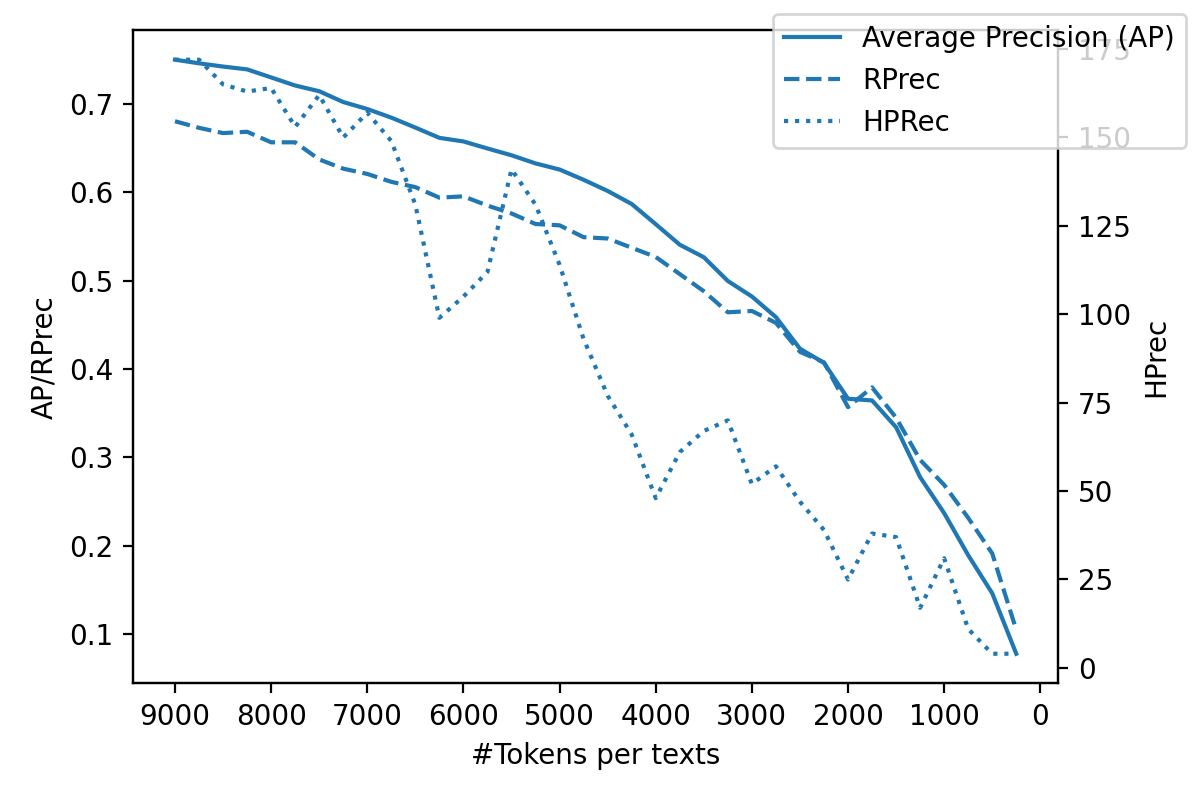
\includegraphics[width=\linewidth]{img/degradation.png}
  \caption{St-Jean ranks list evaluation on AP, RPrec and HPrec over the text size. Rank list computed using 500 MFW and the zscored-normalized cosine distance}
  \label{img:degradation}
\end{figure}

PAN16 dataset is a difficult dataset due to its small size, thus extracting reliable features for each text to estimate each style is also a difficult task.
After multiple tests, the PAN @ CLEF 2016 dataset is not used further in this study due to its difficulty in finding reliable Stylometric clues.

\subsubsection{MFW Token and Lemma}
\label{sec:mfw_token_lemma}

Here the goal is to compare two similar text representations, which are the token representation, words as they appear in the novels, and the lemmatize representation, for example \textit{il voit} (he sees) will be lemmatized to \textit{il voir} (he see).
For this kind of representation, previous studies have shown that using MFW (most frequent words) vector size of around 500 tends to produce better outcomes~\cite{savoy_text_representation}.

After creating the rank lists with the proposed distance measures (ref. Section~\ref{sec:fv_distances}) on the two representations for a MFW vector size ranging between 100 and 2000 with a step of 100, on the two datasets containing the lemmatize representation (Brunet and St-Jean), the two plots in Figure~\ref{fig:token_vs_lemma} show the average precision (AP) for the resulting rank lists.

This representation seem to have good results with a MFW vector size of 500 for most of the metrics, this corroborate previous studies results.
A few metrics, such as Manhattan distance, Tanimoto distance or Clark distance can give better results with slightly bigger vectors.
In most cases, the token representation provide on both dataset a greater average precision compared to the lemma representation.
An interesting example to be worth noticing concern the Manhattan distance, when using the token representation it tends to decrease the AP faster than the lemma representation as the MFW vector size increase.
The euclidean distance seem to be the least appropriate distance measure for this task.
The Clark distance have a really poor average precision when the MFW vector is too small but after reaching 500 it produces one of the best pay-off of the experiment.
Using the most appropriate MFW-vector size for each distance metric, the choice using the right distance metric with these text representations, can increase the average precision by a factor of $13$ to $17$ \% depending on the dataset.
Over all, the cosine distance seem to be one of the most appropriate choice when dealing with these datasets and text representations.

For the next experiments dealing with this text representation, four distance mesures retained : Cosine distance, Clark, Manhattan and Tanimoto, with a MFW vector size of 750.

\begin{figure}
  \centering
  \caption{Token and Lemma representation over number of MFW using different distances metrics}
  \label{fig:token_vs_lemma}

  \subcaption{Brunet}
  \label{fig:token_vs_lemma_brunet}
  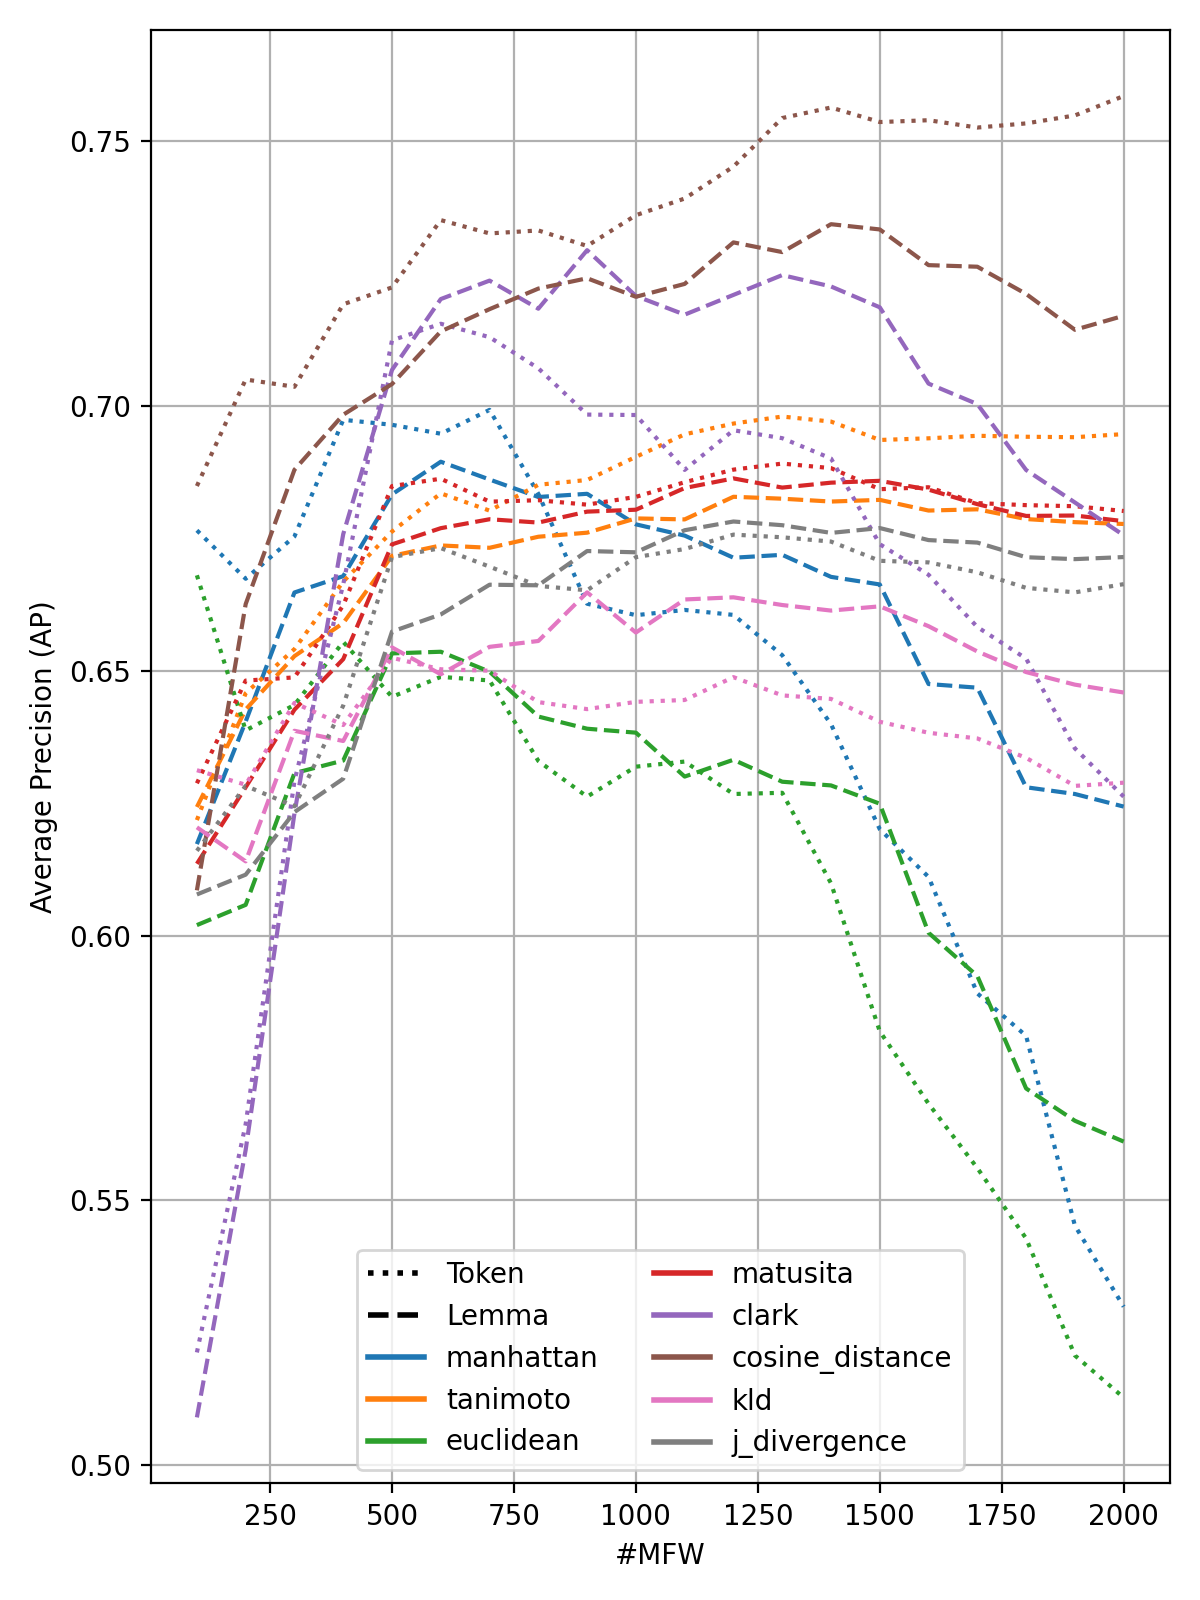
\includegraphics[width=0.9\linewidth]{img/token_vs_lemma_brunet.png}

  \subcaption{St-Jean}
  \label{fig:token_vs_lemma_st_jean}
  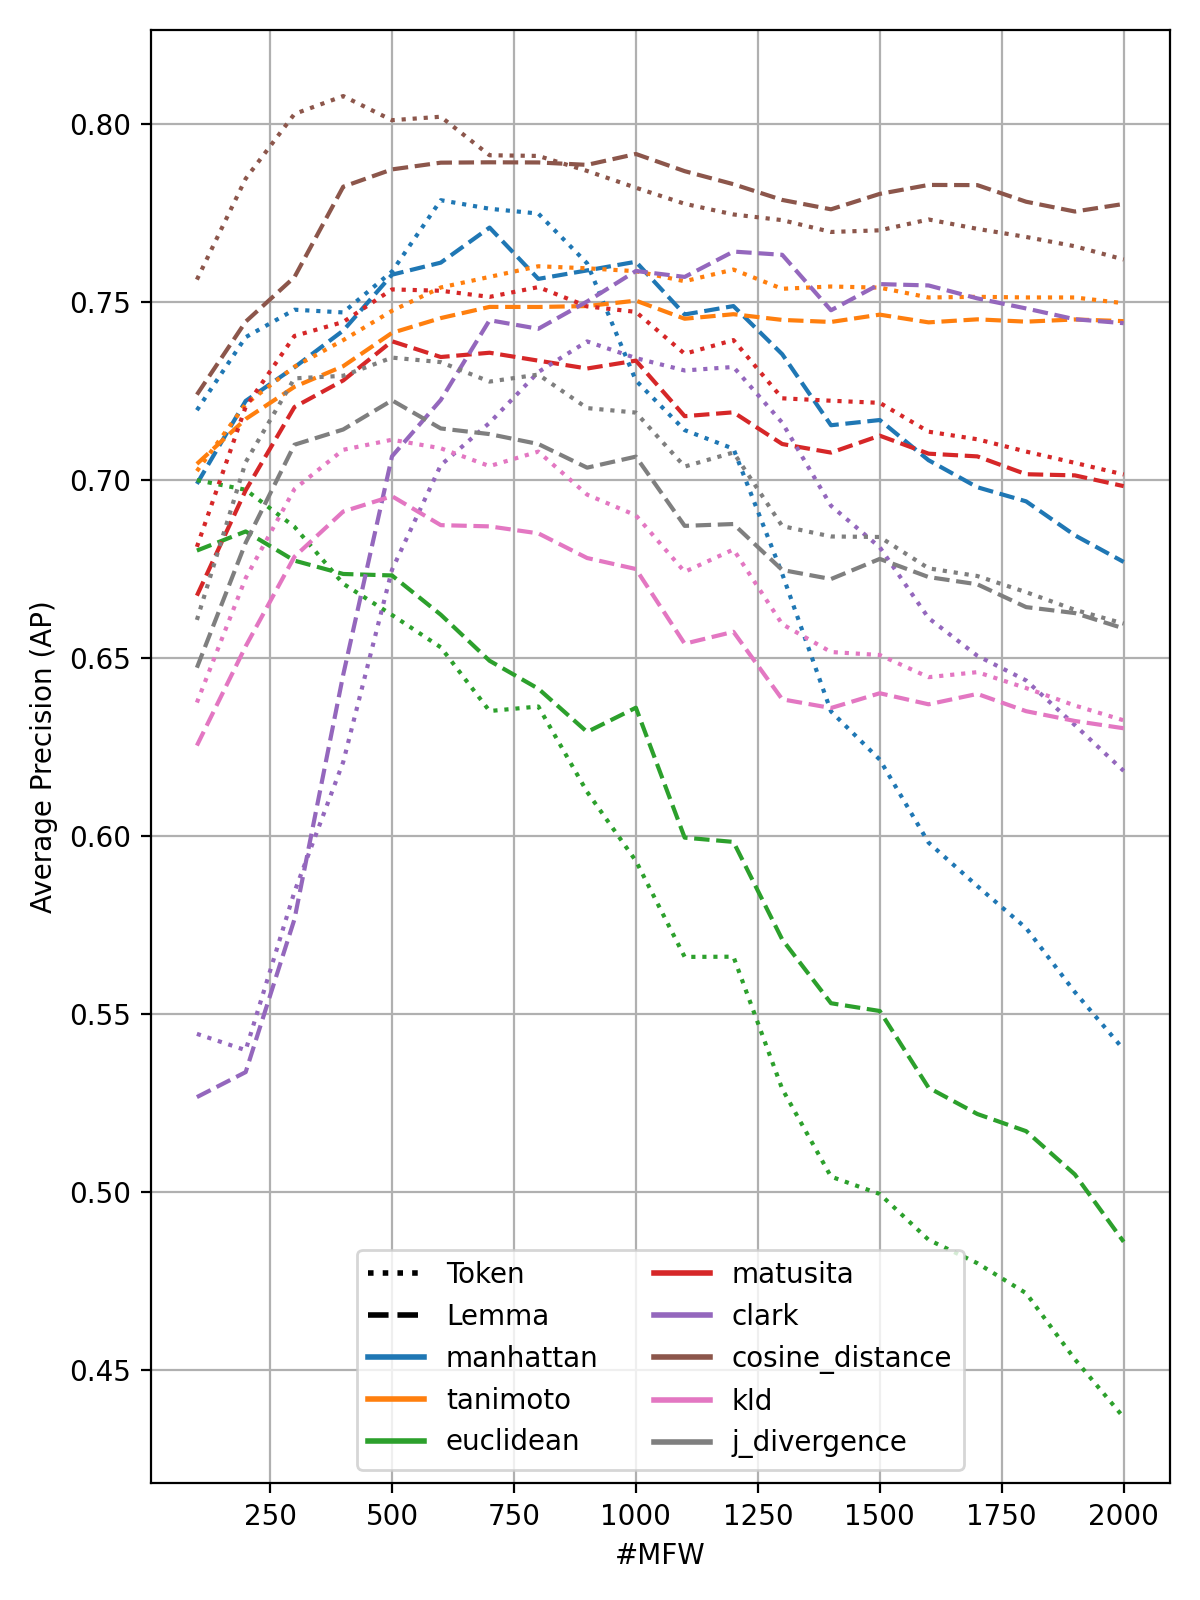
\includegraphics[width=0.9\linewidth]{img/token_vs_lemma_st_jean.png}
\end{figure}

\subsubsection{MFW Letter $n$-grams}

In this experiment the whole text is considered to create letters $n$-grams for the text representation, see Definition~\ref{def:letters_n_grams}.
As for the other experiment the MFW approach is used to create the feature vector.
To reduce the field the possible parameters, the experiment is splited in two parts :
The first part is to find the size of the $n$ parameter of the $n$-grams, and the number of MFW. The second is to compare the distance metrics with the previously found parameters.

\textbf{First Part}\\
For the first part, the z-score normalized cosine distance measure is used to compare the vectors and create the rank list.
The parameters used are: a varying MFW vector size ranging between 500 and 15000 with a step of 500 and a $n$ for the following values : $3, 4, 5, (2, 3), (3, 4), (4, 5)$, the tuples $(a, b)$ correspond to both $a$-grams and $b$-grams in the same text representation.
The number of different $n$-grams is not clear, but it is assumed to be larger than the vocabulary of the texts, thus the importance of having larger vector when dealing with long texts such as the literature datasets.
When considering letters $n$-grams the text representation increase size by a factor of approximately $t$, with $t$ being the average token length.
The average token size for the literature dataset is displayed Table~\ref{tab:lit_datasets}, and is in average $\sim 4$.
To avoid having too large text representation a possible idea is to remove the hapax legomena (tokens appearing only once in the corpus) before applying the $n$-grams algorithm.
This pruning approach was explored in~\cite{kocher_linking} but was not used in this study.

Figure~\ref{fig:letter_ngrams} show the results of the first part of the experiment on the Oxquarry dataset (\ref{fig:letter_ngrams_oxquarry}), Brunet (\ref{fig:letter_ngrams_brunet}) and St-Jean (\ref{fig:letter_ngrams_st_jean}).
The trends seems to indicate that a lower $n$ value converge with lower MFW vector size but reach a maximal value faster.
With $3$-grams, $\sim 3000-4000$-MFW give good results on both datasets with this distance metric.
On the Brunet dataset, after reaching the maximal average precision at $\sim 4000$-MFW, a larger number of frequent words decrease the precision until reaching the maximal number of differant $3$-grams at $\sim 6500$-MFW, which is not the case on Oxquarry.
On St-Jean, the $3$-grams and $(2,3)$-grams don't reach an high average precision with a low number of MFW like for the Brunet and Oxquarry.
$4$-grams also can be efficient but require a larger MFW vector, around $\sim 4000$-MFW give good result for both Brunet and St-Jean but on Oxquarry it requires around $\sim 8000$ to have similar results as the $3000$ $3$-grams.
For the first part, the retained parameters for the $n$-grams text representation are the $3$-grams with $3000$-MFW and $4$-grams with $8000$-MFW.

\begin{figure}
  \caption{Letters $n$-grams representation over number of MFW with different $n$}
  \label{fig:letter_ngrams}

  \subcaption{Oxquarry}
  \label{fig:letter_ngrams_oxquarry}
  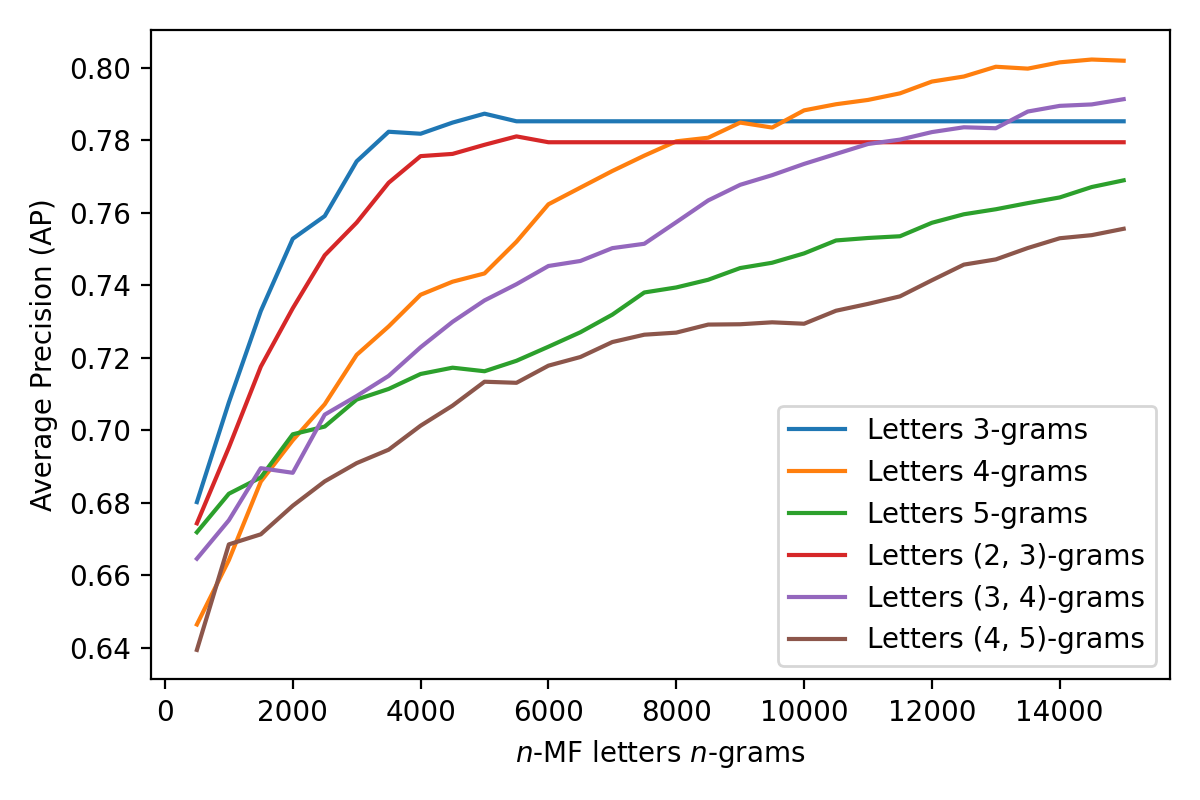
\includegraphics[width=\linewidth]{img/letter_ngrams_oxquarry.png}

  \subcaption{Brunet}
  \label{fig:letter_ngrams_brunet}
  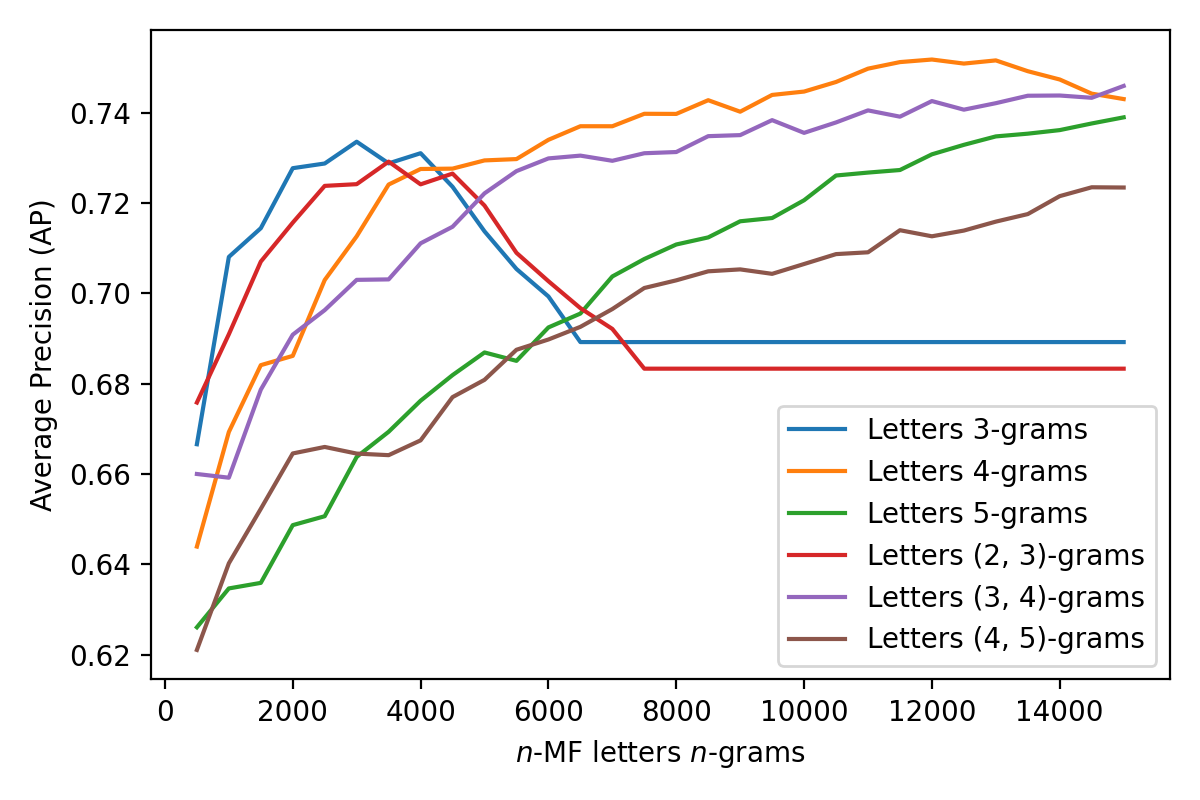
\includegraphics[width=\linewidth]{img/letter_ngrams_brunet.png}

  \subcaption{St-Jean}
  \label{fig:letter_ngrams_st_jean}
  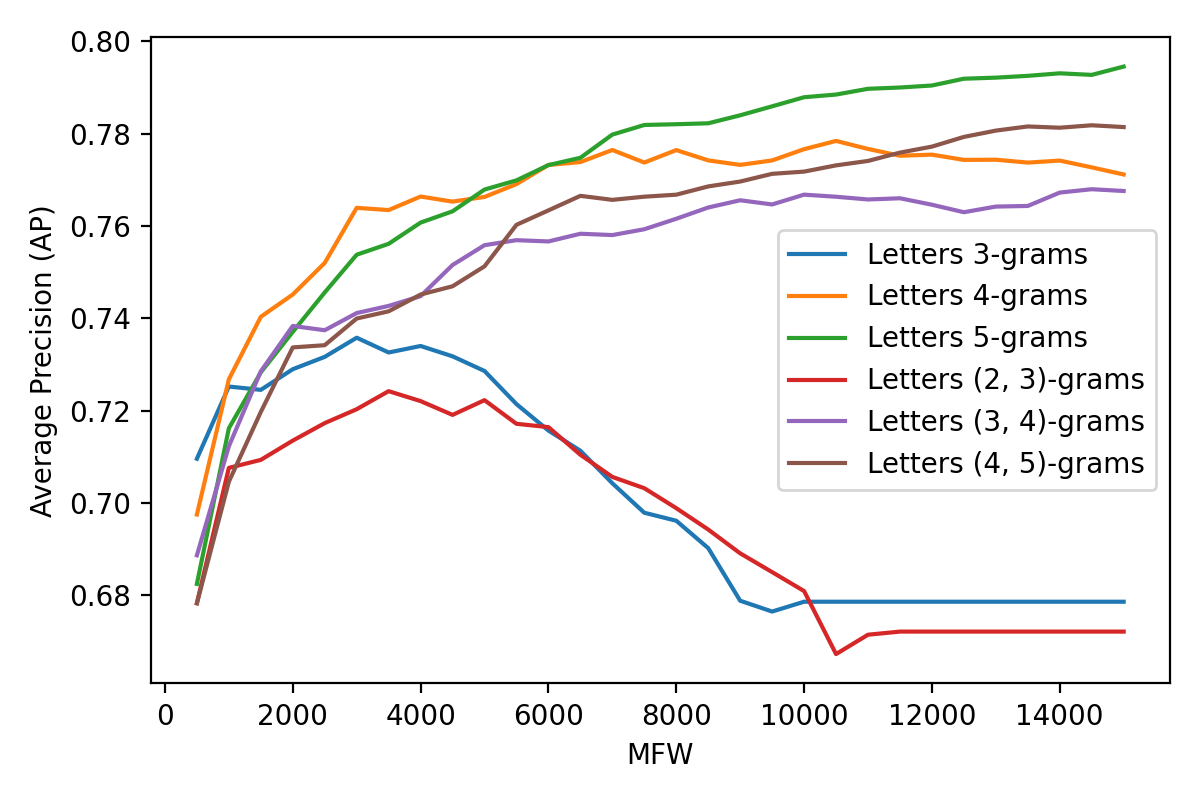
\includegraphics[width=\linewidth]{img/letter_ngrams_st_jean.png}
\end{figure}

\textbf{Second Part}\\
As stated earlier, in the second part the objective it to compare the distance metrics with the $3$-grams/$3000$-MFW and $4$-grams/$8000$-MFW.
The distance metrics used are the ones presented in Section~\ref{sec:fv_distances}.
The results for this experiment are in Table~\ref{tab:letter_ngrams}.
Since the number of MFW and the size of the $n$-grams was optimized on the cosine distance, the results may be biased.

For the $3$-grams, the following results can be observed:
The cosine distance give the best results.
Though two distances metrics can compete with the cosine distance on certain datasets with the $3$-grams approach, namely the Manhattan distance and the Clark distance.
A worth noticing results, is the euclidean distance, which have polarized results: on Oxquarry the average precision is $0.72$ and on St-Jean only $0.47$.
Using the right distance measure can have a relative increase up to $36$\%, when comparing the worse distance metric to the best of each dataset.

For the $4$-grams approach, as for the $3$-grams the cosine is the best measure with this configuration.
The Manhattan distance and the Clark distance also are the second choice.
The euclidean have the same behavior as for $3$-grams on the dataset.
For this configuration of $4$-grams with $8000$-MFW, using the right distance measure is less impactful than the $3$-grams approach but still can have a relative increase in  performance of $28$\% when changing from the worse distance metric to the best, with these datasets.

\begin{table}
  \centering
  \caption{Average precision for $n$-grams with every metrics, on the 3 datasets (best result for the dataset in bold).}
  \label{tab:letter_ngrams}

  \subcaption{$3$-grams with $3000$-MFW}
  \begin{tabular}{l c c c}
    \toprule
    Distance metric & Oxquarry & Brunet & St-Jean \\
    \midrule
    Manhattan & \textbf{0.77} & 0.66 & 0.62 \\
    Tanimoto & 0.64 & 0.66 & 0.62 \\
    Euclidean & 0.72 & 0.63 & 0.47 \\
    Matusita & 0.60 & 0.66 & 0.58 \\
    Clark & 0.64 & \textbf{0.73} & 0.63 \\
    Cosine & \textbf{0.77} & \textbf{0.73} & \textbf{0.74} \\
    KLD & 0.57 & 0.65 & 0.54 \\
    JD & 0.58 & 0.66 & 0.56 \\
    \bottomrule
  \end{tabular}

  \subcaption{$4$-grams with $8000$-MFW}
  \begin{tabular}{l c c c}
    \toprule
    Distance metric & Oxquarry & Brunet & St-Jean \\
    \midrule
    Manhattan & 0.76 & 0.69 & 0.73 \\
    Tanimoto & 0.68 & 0.68 & 0.68 \\
    Euclidean & 0.73 & 0.65 & 0.55 \\
    Matusita & 0.63 & 0.68 & 0.65 \\
    Clark & 0.67 & 0.72 & 0.75 \\
    Cosine & \textbf{0.78} & \textbf{0.74} & \textbf{0.78} \\
    KLD & 0.61 & 0.66 & 0.60 \\
    JD & 0.61 & 0.67 & 0.63 \\
    \bottomrule
  \end{tabular}
\end{table}


\subsubsection{MFW First letters, last letters, word n-grams of tokens}

In this experiment, the goal is to create 3 types of text representations of word substrings and compare them.

\begin{enumerate}
  \item
  The first representation is the N-first letter of each word tokens which correspond generally to the meaning of a word.
  If the word token is smaller than N, the whole word is used.
  \item
  Extract also the N-last letter of each word tokens which in this case correspond to the role of the word in a sentence.
  As for the previous representation, if the word is smaller than N, the whole is used instead.
  \item
  The in-word $n$-grams (See Definition~\ref{def:words_n_grams}), this special type of n-grams consider only $n$-grams within a word.
  This excludes every overlapping word when considering the Letters $n$-grams algorithm.
  This decision is made for this experiment such that interwords style information can't be learned and have a fair comparison of these 3 texts representations.
\end{enumerate}

The first approach can be related to the lemma approach, the second to the POS approach and the third to a hybrid version between the letters $n$-grams and the word token text representations.
The two first representations have the same number of words as the token text representation.
The third representation is smaller than the Letters $n$-grams text representation.
The two first representation are subsets of the third method.

For this experiment the only distance measure used is the z-normalized cosine distance and, for the evaluation metric only the average precision.
The number of MFW variate for this experiment between 200 and 4000 with a step of 100.
Figure~\ref{fig:first_last_letters_ngrams_brunet} shows the results for the Brunet dataset and Figure~\ref{fig:first_last_letters_ngrams_oxquarry} for the Oxquarry dataset.

\begin{figure}
  \centering
  \caption{Average precision over the MFW in the rank list generated using the z-score normalized cosine distance}

  \subcaption{Oxquarry}
  \label{fig:first_last_letters_ngrams_oxquarry}
  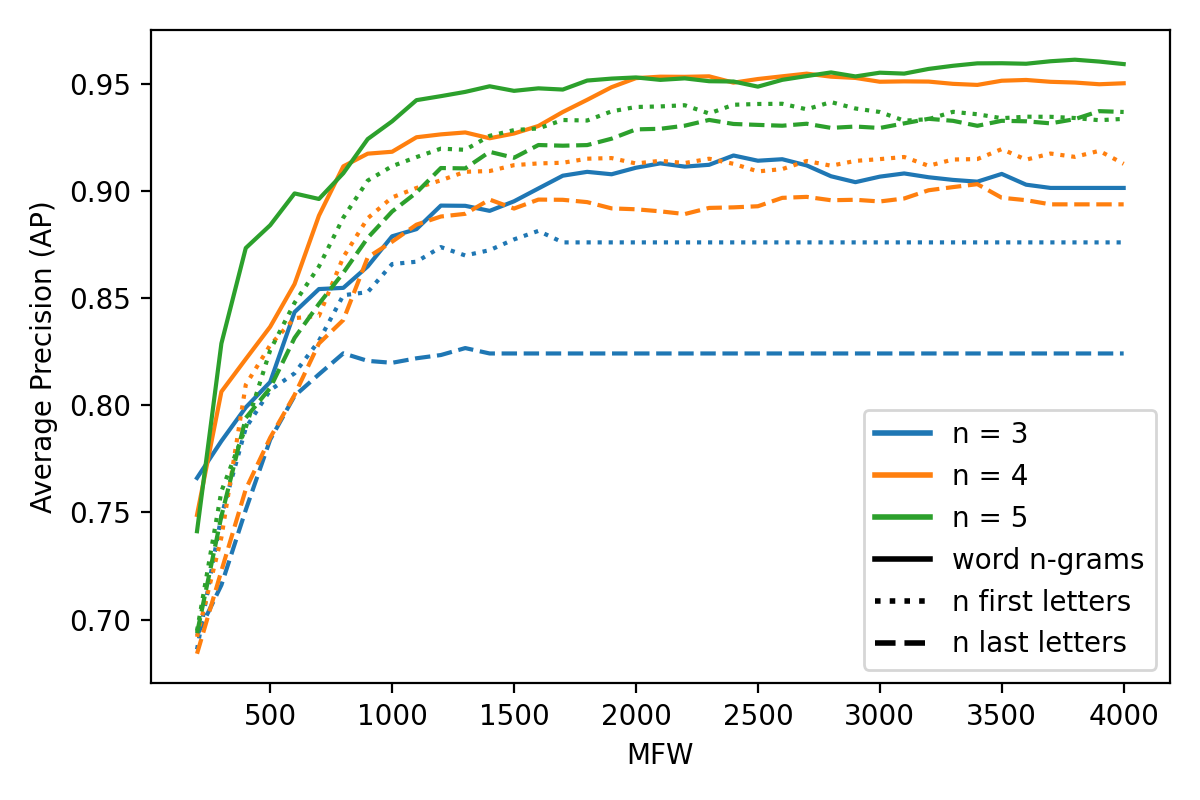
\includegraphics[width=\linewidth]{img/first_last_letters_ngrams_oxquarry.png}

  \subcaption{Brunet}
  \label{fig:first_last_letters_ngrams_brunet}
  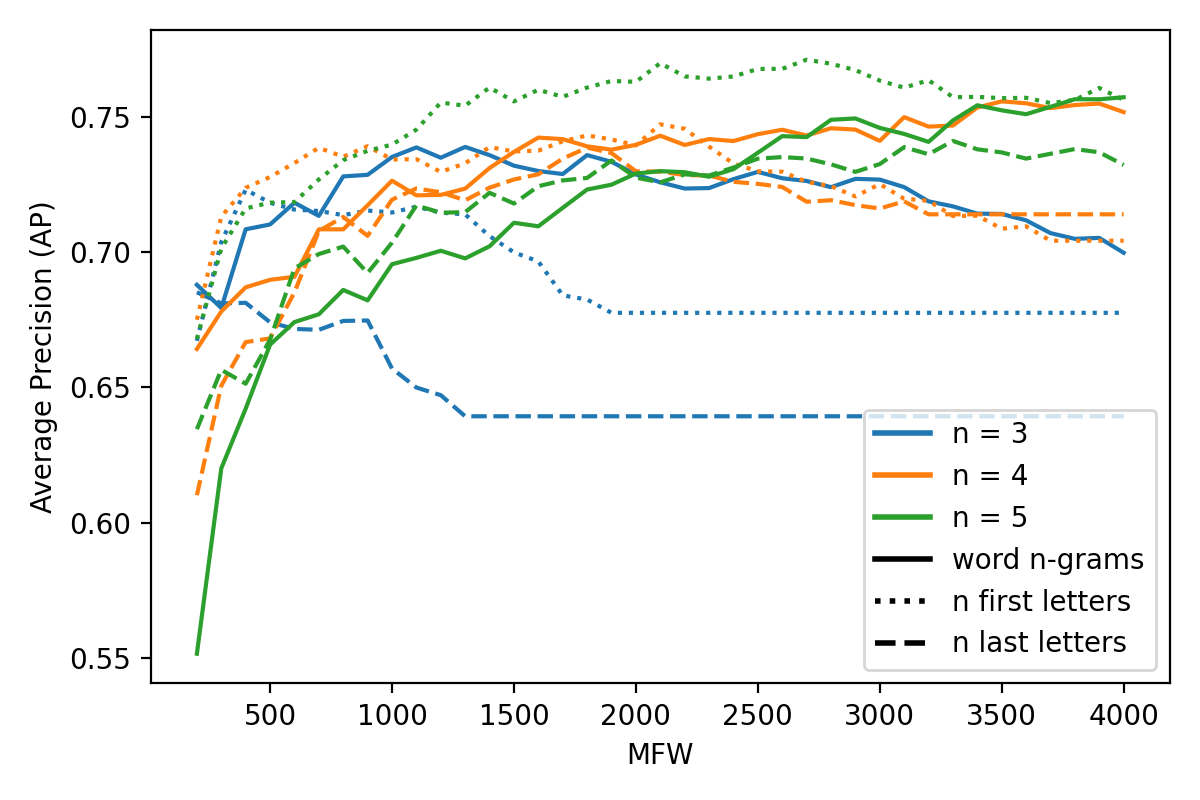
\includegraphics[width=\linewidth]{img/first_last_letters_ngrams_brunet.png}
\end{figure}

In both dataset, the 3-last letters and 3-first letters gives a lower average precision and quickly converge to an equilibrium value at around 1500 MFW.
5-letters representations tend to produce better results than 3-letters and 4-letters representation as the MFW increase.
In the Oxquarry corpus, word 4-grams and word 5-grams give the best results with an average precision of ~95.0\%, but is not as efficient for the Brunet dataset.
For the Brunet dataset, the 5-first letters can a good results compared to other text representations with small MFW vector size.

For this experiment, no metrics was retained for the fusion, since the results are mixed.

\subsubsection{MFW POS $n$-grams}

For this experiment short combination of POS are used to detect the style of the author.
POS $1$-grams are not test (equivalent of the POS frequency) since previous studies showed that POS $1$-grams tends to produce worse results then POS $2$/$3$/$4$-grams~\cite{kocher_linking}.
The St-Jean dataset have for every word a POS tag, by using these POS tags and combining them using Definition~\ref{def:letters_n_grams} to create $n$-grams/w-shingling, a new text representation is obtained.
Using this representation the $n$-MFW are computed and the rank list containing every document pairs can be computed.

In this experiment, only $2$-grams, $3$-grams, $4$-grams and the combination of the $2$-grams and $3$-grams denoted: $(2, 3)$-grams is used.
The distance metric used is the smoothed z-score normalized cosine distance.
For this representation no clear MFW (most frequent word, in this case POS $n$-grams are considered as words) vector size is advised, the size used is between 200 and 2000 with a step of 100.
Figure~\ref{fig:pos_ngrams} show the average precision on the rank list produced by using POS $n$-grams over the number of MFW.

The two following information can be intuitively observed on this plot:
\begin{itemize}
  \item
  A more complex POS $n$-grams require more MFW to archive its maximal effectiveness.
  In the St-Jean corpus, 26 POS are used to describe every words in the corpus.
  Which correspond to $26^2 = 676$ possible unique POS $2$-grams, to $26^3 = 17'576$ POS $3$-grams and $26^4 = 456'976$ POS $4$-grams, thus the the convergence of $2$-grams and not $3$/$4$-grams.
  \item
  Like other methods, if the MFW ceiling is too high, an overfitting to less important words is possible, thus reducing the average precision.
  In Figure~\ref{fig:pos_ngrams} the POS 2-grams clearly have a drop in average precision after $\sim 250$-MFW.
\end{itemize}

Using the smoothed z-score cosine distance, the most appropriate configuration for the POS $n$-grams text representation on St-Jean seem to be 250 MFW POS $2$-grams and 1000 MFW POS $3$-grams.
These two methods are kept for the fusion.

\begin{figure}
  \centering
  \caption{Average precision over the MFW in the rank list generated using the z-score normalized cosine distance on St-Jean POS n-grams text representation.}
  \label{fig:pos_ngrams}
  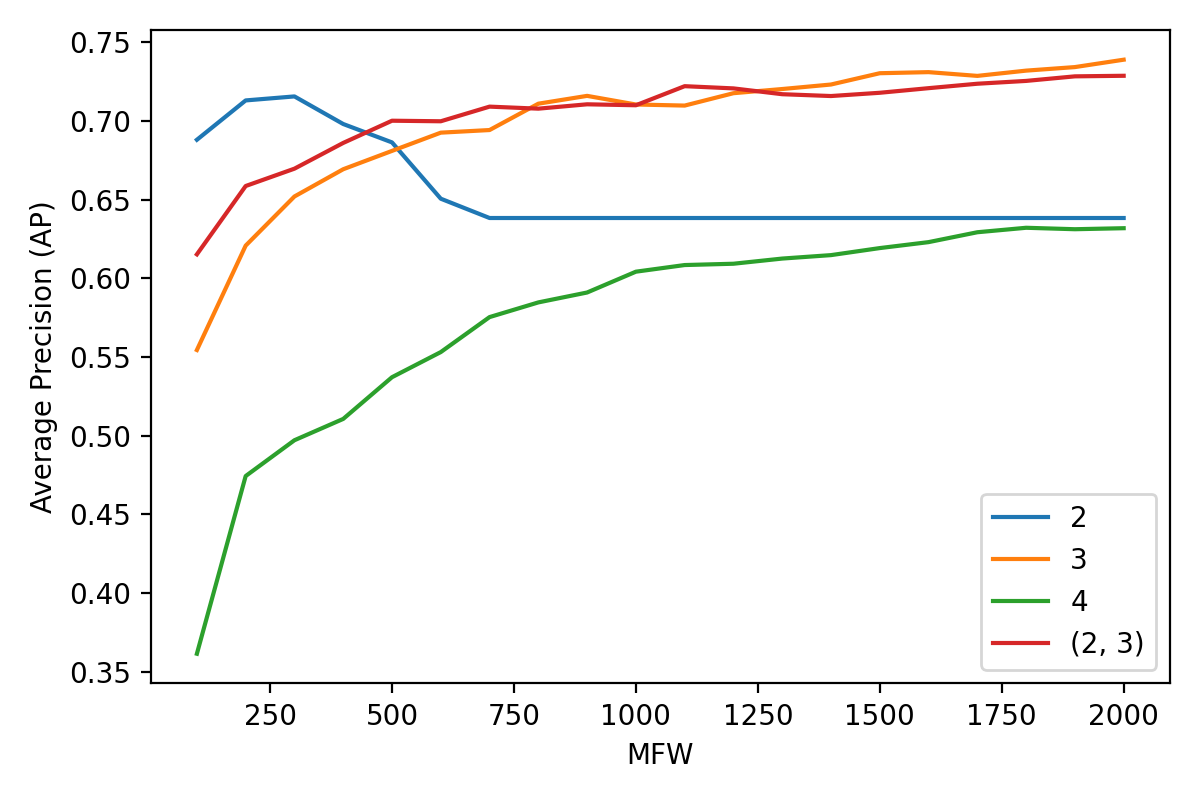
\includegraphics[width=\linewidth]{img/pos_ngrams.png}
\end{figure}

\subsubsection{Compression based distances}

This experiment try to compare the three proposed compression algorithm (GZip, BZip2, LZMA) for the compression based distance ranking.
For each algorithm and for each document, the size after compression is computed, as well as the concatenation of every document pairs.
Using these sizes and the NCD or CBC distance metrics (ref. Section~\ref{sec:compression_based_distances}, the rank list is evaluated.
This experiment is run on the three datasets three times to have a better approximation of the run time.
The results in terms of efficiency of the resulting rank list are shown in Table~\ref{tab:compression_evaluation_results}.
The average time of the three runs are in Table~\ref{tab:compression_evaluation_times} when run on a Intel(R) Core(TM) i7-5820K CPU @ 3.30GHz.

GZip seem to be giving the worse results on every dataset with an average AP of $\sim -0.20$ in compared to LZMA and BZip2.
LZMA give the best results on every dataset tested, but BZip2 have close results.
The cosine-based compression distance (CBC) tend to give better results over the normalized compression distance (NCD).
In terms of time complexity BZip2 is the fastest algorithm of the 3 proposed, LZMA is $\sim ~5-6$ times slower than BZip2, and GZip slower than BZip2 by around $\sim 5-20$\%.
No significant time differences is recorded between the NCD and CBC distance measures, since the greatest complexity reside in the compression algorithm.
Even though LZMA algorithm give the best results, the configuration retained for the compression based distance is the BZip2 with the Cosine based compression distance, since it gives relative good results in a short amount of time.

For this text representation the retained configuration is the BZip2 algorithm with the CBC distance measure.
The Bzip2 was selected even though LZMA give slightly better results, due to the huge difference in run time.

\begin{table}
  \centering
  \caption{Evaluation of the different compression algorithm and distance metrics using Average Precision (AP), R-Precision (RP) and High Precision (HP)}
  \label{tab:compression_evaluation_results}

  \subcaption{Oxquarry}
  \label{tab:compression_evaluation_oxquarry}
  \begin{tabular}{l c c}
    \toprule
    AP/RPrec/HPrec & NCD          & CBC \\
    \midrule
    Bzip2          & 0.77/0.68/69 & 0.79/0.69/74 \\
    GZip           & 0.62/0.56/41 & 0.64/0.56/43 \\
    LZMA           & 0.81/0.70/82 & 0.84/0.73/85 \\
    \bottomrule
  \end{tabular}

  \subcaption{Brunet}
  \label{tab:compression_evaluation_brunet}
  \begin{tabular}{l c c}
    \toprule
    AP/RPrec/HPrec & NCD          & CBC \\
    \midrule
    Bzip2          & 0.76/0.70/25 & 0.76/0.70/25 \\
    GZip           & 0.61/0.53/24 & 0.60/0.52/23 \\
    LZMA           & 0.78/0.73/27 & 0.79/0.73/31 \\
    \bottomrule
  \end{tabular}

  \subcaption{St-Jean}
  \label{tab:compression_evaluation_st_jean}
  \begin{tabular}{l c c}
    \toprule
    AP/RPrec/HPrec & NCD           & CBC \\
    \midrule
    Bzip2          & 0.70/0.63/214 & 0.70/0.62/219 \\
    GZip           & 0.45/0.44/54  & 0.42/0.42/56 \\
    LZMA           & 0.71/0.63/241 & 0.71/0.62/214 \\
    \bottomrule
  \end{tabular}
\end{table}

\begin{table}
  \centering
  \caption{Average run time for the rank list computation with the different compression algorithm and distance metrics}
  \label{tab:compression_evaluation_times}

  \subcaption{Oxquarry}
  \label{tab:compression_evaluation_time_oxquarry}
  \begin{tabular}{l c c}
    \toprule
    Time      & NCD   & CBC \\
    \midrule
    Bzip2     & 12.7s & 12.7s \\
    GZip      & 15.0s & 14.9s \\
    LZMA      & 69.0s & 68.8s \\
    \bottomrule
  \end{tabular}

  \subcaption{Brunet}
  \label{tab:compression_evaluation_time_brunet}
  \begin{tabular}{l c c}
    \toprule
    Time      & NCD   & CBC \\
    \midrule
    Bzip2     & 8.4s & 8.4s \\
    GZip      & 8.8s & 8.9s \\
    LZMA      & 46.6s & 46.8s \\
    \bottomrule
  \end{tabular}

  \subcaption{St-Jean}
  \label{tab:compression_evaluation_time_st_jean}
  \begin{tabular}{l c c}
    \toprule
    Time      & NCD    & CBC \\
    \midrule
    Bzip2     & 198.9s  & 198.4s \\
    GZip      & 211.3s  & 214.5s \\
    LZMA      & 1046.3s & 1052.0s \\
    \bottomrule
  \end{tabular}
\end{table}

\subsection{Errors analysis}

This section aim to understand the errors of the system, provide potential cues to solve them.

\subsubsection{Frequent errors}
\label{sec:frequent_errors}

This section try to understand the errors in the system, in this case the false links (document pairs with different authors) highly ranked on different rank lists.
The rank list quality is highly based on the feature vector created using the $n$-MFW, having a good understanding of this vector give good indications of the strength of the system.

To find recurrent errors in the system, the retained methods in Section~\ref{sec:mfw_token_lemma} on the relative frequency of the 750-MFW using the whole St-Jean dataset.
This generates the 9 rank lists, presented in Table~\ref{tab:9rl_results_st_jean_A_B} in annex.
For the sake of this experiment, every true links are discarded in the rank lists.
Links often apearing in the top 30 false links are considered as frequent errors.
The goal is to compare the two feature vectors of the frequent errors.
In this case, the visualization is based on the 750-MFW tokens representation.
Figures~\ref{fig:mfw_vector_error} show two pairs (document 57 from Sand / document 183 from Stael and document 57 from Sand / document 141 from Stael) that appear 6 time out of the 9 rank lists in the top 30 false links.
To be able to understand more easily this vector, the values have been sorted by relative frequencies and using the logarithmic scale.
When a large proportion of the vectors overlap it indicates a high similarity between the MFW vectors.

\begin{figure}
  \centering
  \caption{Example of 750-MFW relative frequency vectors for the two documents in a reccurant (6 rank lists out of 9) false link in the top 30 false links}
  \label{fig:mfw_vector_error}

  \subcaption{First example}
  \label{fig:mfw_vector_error_0}
  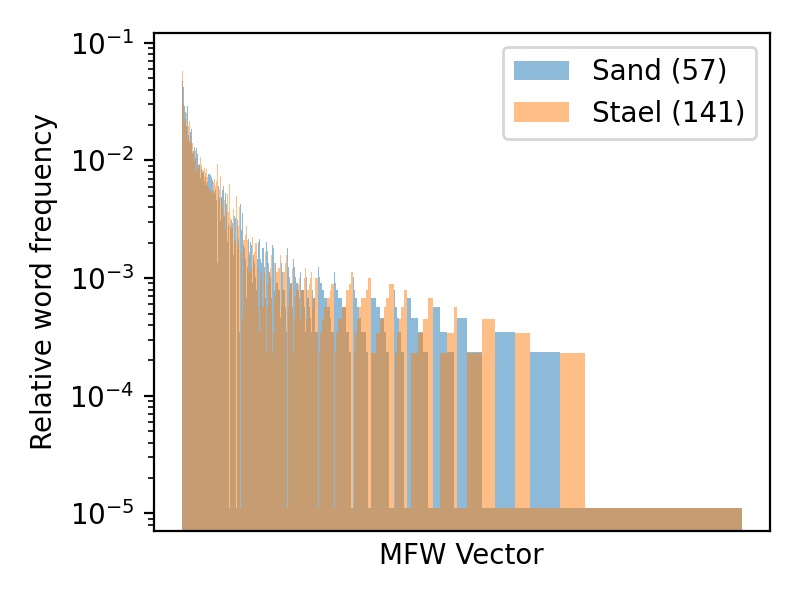
\includegraphics[width=\linewidth]{img/mfw_vector_error_0.png}

  \subcaption{Second example}
  \label{fig:mfw_vector_error_1}
  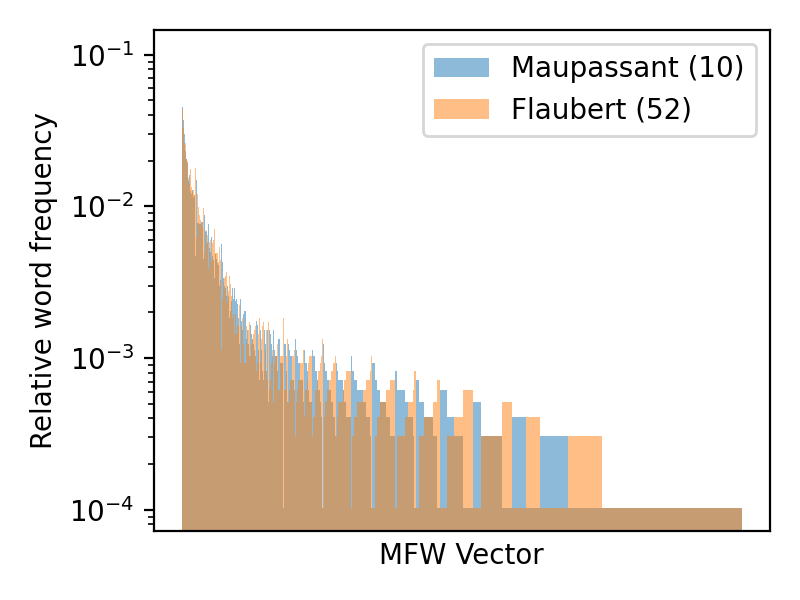
\includegraphics[width=\linewidth]{img/mfw_vector_error_1.png}
\end{figure}

Both document style are close when their feature vector are closely related.
Visually when most the surface overlap, the distance function will give a low value, and rank this link high in the list.
When two vectors are relatively close together determinating that two texts are from a different author can not clearly be established using only one type of representation, no matter the distance metric applied.
The frequent errors vector pairs presented in Figure~\ref{fig:mfw_vector_error} can be visually compared actual true links and actual false links, to have a better understanding of this problematic.
For example the most similar true link (ranked 1 using Manhattan distance) in Figure~\ref{fig:mfw_vector_first_rl} (document 157 from Stael / document 183 from Steal) or the HPrec-th (last continous correct pair from the top of the list) in Figure~\ref{fig:mfw_vector_first_last_rl} (document 4 from Flaubert / document 82 from Flaubert), both of these links show a large proportion of overlapping surface, like for the frequent errors vectors.
A counter example would be the least similar false link (ranked last using Manhattan distance) which represent a negatively correlated document pair, Figure~\ref{fig:mfw_vector_last_rl} showcase this link (document 92 from Zola / document 191 from Stael).
As expected, most of this figure surface is non-overlapping.

\begin{figure}
  \centering
  \caption{750-MFW relative frequency for the two documents ranked $X$ in the rank list using the token representation on St-Jean}

  \subcaption{$X$ = First}
  \label{fig:mfw_vector_first_rl}
  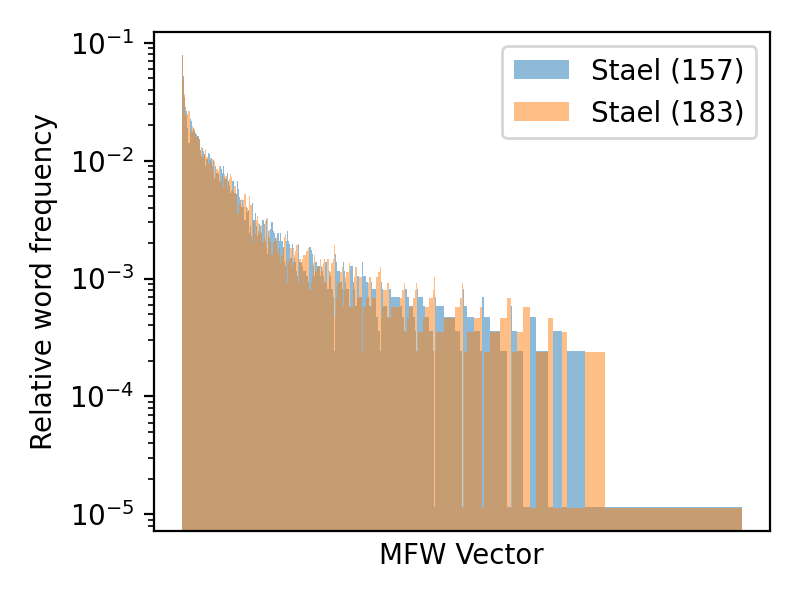
\includegraphics[width=\linewidth]{img/mfw_vector_first_rl.png}

  \subcaption{$X$ = HPrec-th}
  \label{fig:mfw_vector_first_last_rl}
  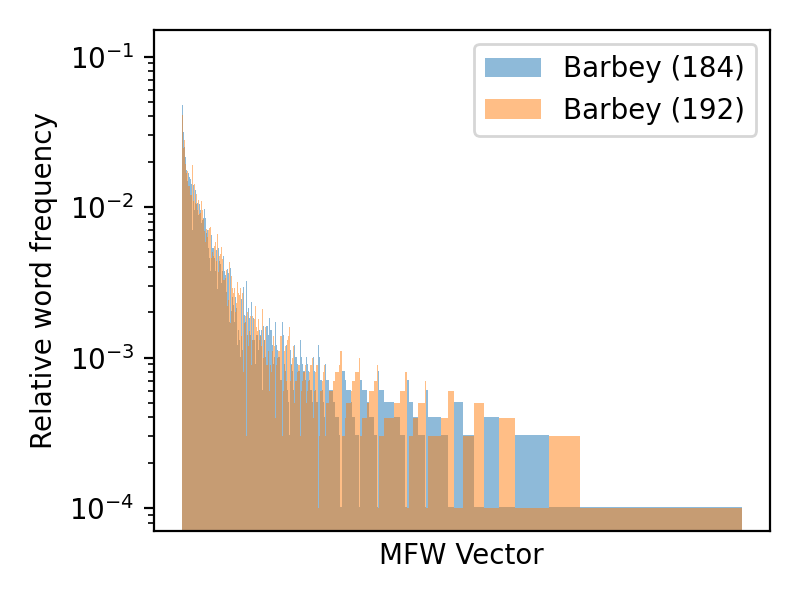
\includegraphics[width=\linewidth]{img/mfw_vector_first_last_rl.png}

  \subcaption{$X$ = Last}
  \label{fig:mfw_vector_last_rl}
  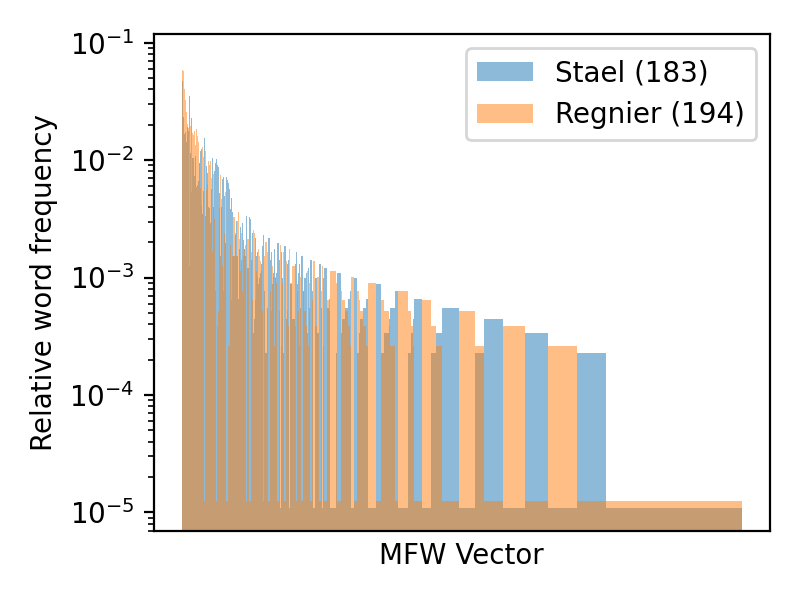
\includegraphics[width=\linewidth]{img/mfw_vector_last_rl.png}
\end{figure}

\subsubsection{Publication date differences analyis}

When dealing with false links ranked high in the rank list, as the previous experiment showed, some excerpt use similar words.
These shared words might be related to the era the book was written in.
The following experiment try to investigate on this.

In the St-Jean dataset publication paper, the publication dates of each excepts are available~\cite{st_jean}.
First the publication date distribution of the dataset must be understood.
Figure~\ref{fig:dates_distribution} show the distribution of the publication date in the St-Jean dataset.
The date difference distribution for each pair of documents can be computed, Figure~\ref{fig:dates_differences_all} showcase this.
The average date difference in the dataset is 28.24 years with a standard deviation of 20.73 years.
Since this dataset contain multiple excerpt from the same book, considering only the links of different authors (false links) is preferable.
Figure~\ref{fig:dates_differences_false} shows the date difference distribution of the false links.
As expected the mean increased from 28.24 years to 29.04 years since there are fewer links with small date difference.
Same authors links (true links) are displayed in Figure~\ref{fig:dates_differences_r_true}, they confirm the previous statement that most of the same authors links have a low date difference with a mean of 5.11 years.

\begin{figure}
  \centering
  \caption{Dates and Date differences denstiy distributions on St-Jean for every excerpt}

  \subcaption{Date distribution}
  \label{fig:dates_distribution}
  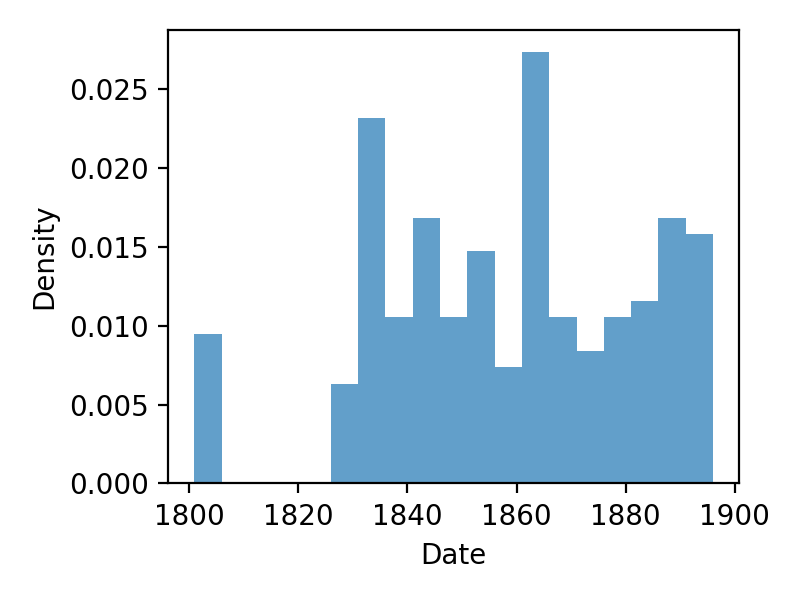
\includegraphics[width=\linewidth]{img/dates_distribution.png}

  \subcaption{Date difference denstiy distributions}
  \label{fig:dates_differences_all}
  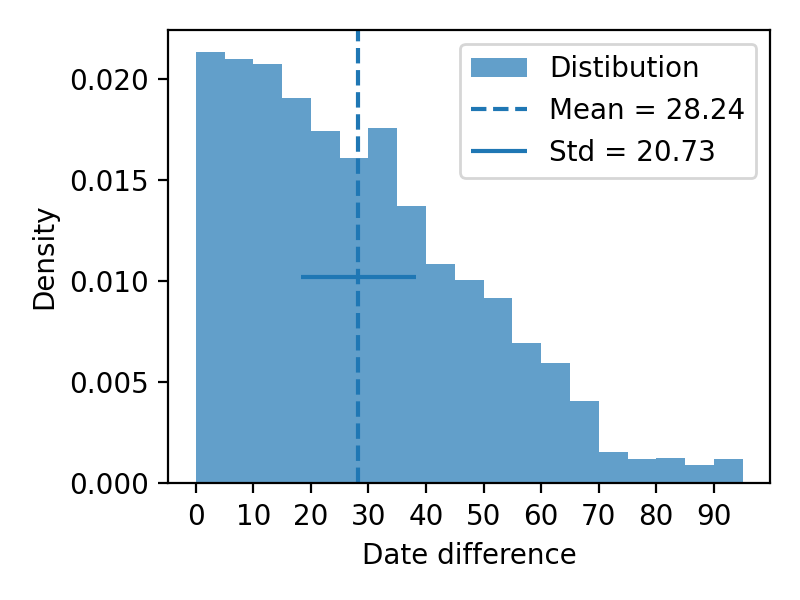
\includegraphics[width=\linewidth]{img/dates_differences_all.png}
\end{figure}

\begin{figure}
  \centering
  \caption{Date difference denstiy distributions in St-Jean}

  \subcaption{False links}
  \label{fig:dates_differences_false}
  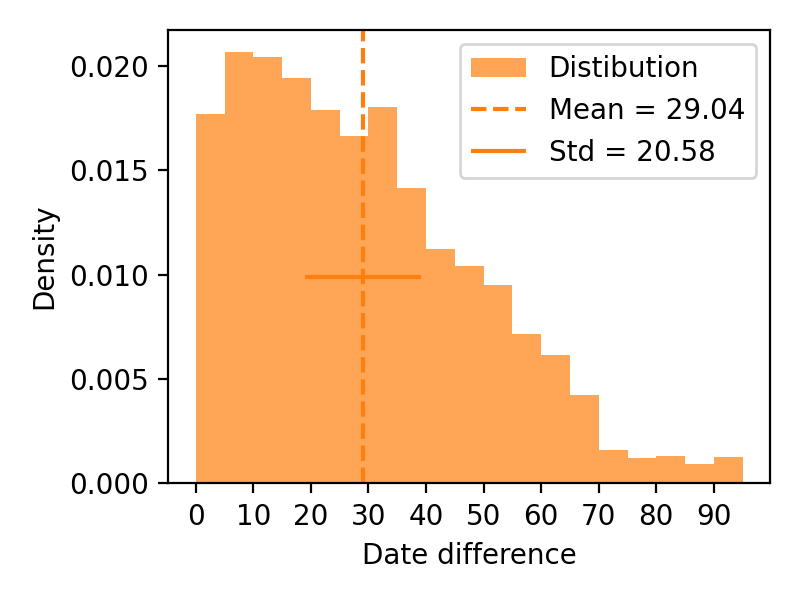
\includegraphics[width=\linewidth]{img/dates_differences_false.png}

  \subcaption{True links}
  \label{fig:dates_differences_r_true}
  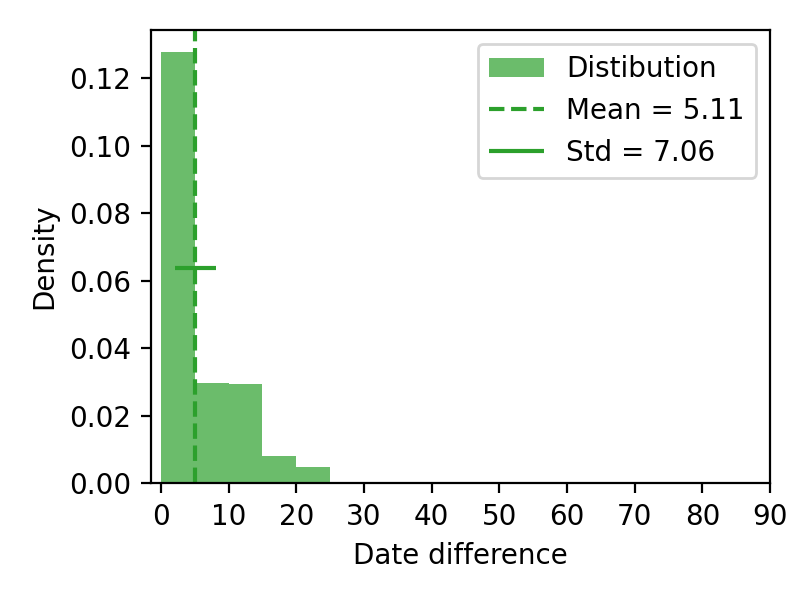
\includegraphics[width=\linewidth]{img/dates_differences_r_true.png}

  \subcaption{Top-r false links using a rank list with 85\% average precision.}
  \label{fig:dates_differences_r_false}
  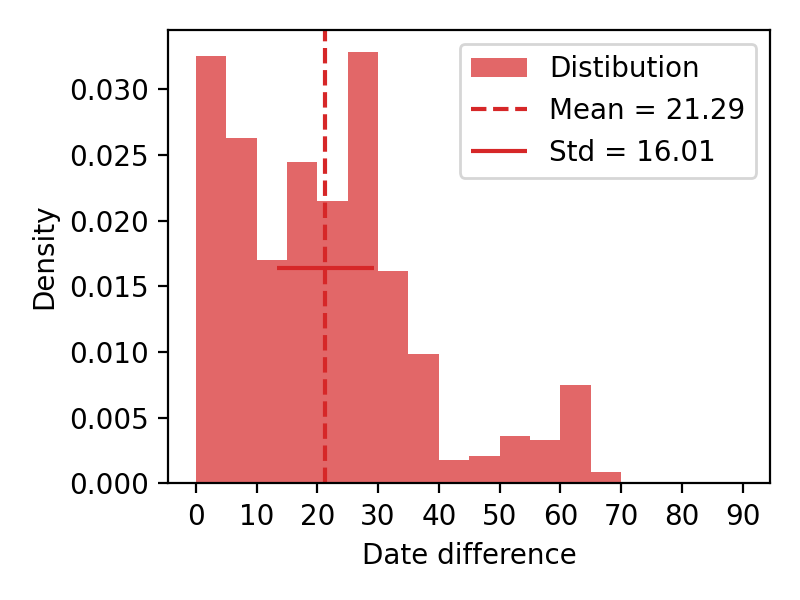
\includegraphics[width=\linewidth]{img/dates_differences_r_false.png}
\end{figure}

The previous statistics can be compared to Figure~\ref{fig:dates_differences_r_false} which show the date difference density on the top-r false links (670 in case of St-Jean) on a rank list with 85\% average precision (z-score fusion of the retained text representations, Table~\ref{tab:9rl_results_st_jean_A_B}).
Two interesting information can be extracted here.
First the mean is lower by 7.44 years (29.04 - 21.60) compared to the false links and have a narrow standard deviation distribution which clearly indicate the importance of publication date in the ranking of the documents.
Secondly we can observe a drop after 35 years of date difference, which indicate that links in the interval $\left[0-35\right]$ years are harder to discriminate between a true link and a false link than links outside this interval.
This 35 years interval can be related to the generation factor, the age of woman giving birth is around 25-34 in France~\cite{generations}, the birth country of the authors in this dataset.
Each new generation tend to use its own vocabulary, and thus it can be harder to discriminate the author of text belonging to the same generation, if we assume that the authors write their books at around the same age.
In the other hand having different vocabulary can indicate a different time period and is often used to detect document forgery~\cite{savoy_stylo}.

\subsection{Rank lists fusion evaluation \label{sec:eval_fusion}}

In this experiment, the goal to understand if fusing rank list can improve performance of the rank list.
The methodology used, is to create $n$ rank lists and fuse them for every $r$ rank lists combinations ($C^n_r$) for the two fusing methods proposed, z-score fusion and regression fusion.

The rank list used are the ones obtained by using the 9 retained rank list methods ($n=9$), see Table~\ref{tab:9rl} in annex.
They represent the best configuration retained for each text representation.
The $r$ value is selected to $4$, since it represents the number of different text representation.
The number of possible fusion combinations is with $n=9$ and $r=4$ is $C^{9}_{4} = 126$.
For this 126 fusions, the 3 metrics: Average Precision (AP), R-Precision (RPrec) and High Precision (HPrec) are computed.

To compare the rank list produced by both the Z-Score fusions and the Regression fusion to the non-fused rank lists, two evaluation strategies are used.
One called \textit{Single-Max} which represent the best metrics for each rank list in the fusion and another one called \textit{Single-Mean} which is represented by the mean of each rank list metrics in the fusion.
For example, if for a fusion the average precision of the 4 rank lists are : $0.5, 0.6, 0.7, 0.8$. Single-mean would have an average precision of $0.65$ and Single-max an average precision of $0.8$.
If the Single-Max evaluation strategy is over-come by a rank list produced by a fusion it means that the resulting rank list give results even better then every individual rank lists used for this fusion, the best case.
For the Single-Mean, if it is over come it means that the obtained rank list have better results than the average results of the rank list, thus when using the system \textit{in the blind} (when the rank list can't be evaluated, with new data for example), fusing is a good approach since it gives stability.

The results of every fusion combinations using the proposed rank list and strategies are graphically presented in Figure~\ref{fig:fusions}.
Statistiques for each metrics and fusion schemes are resumed Tables~\ref{tab:fusion_stats_A_B}/\ref{tab:fusion_stats_B_A}, it contains for each metric, the minimal value (min), the average and the standard deviation (Avg$\pm$Std), the maximal value, the argmin and argmax for the metrics (using ids of the rank list in Table~\ref{tab:9rl} in annex).
A sign test between the two strategies and the two fusion methods is presented in Table~\ref{tab:fusion_sign_test}.

\begin{figure}
  \centering
  \caption{Evaluation of every combination of 4 rank list fusions using Z-Score and Regression}
  \label{fig:fusions}

  \subcaption{Testing on St-Jean A (training St-Jean B, for the Regression fusion)}
  \label{fig:fusion_B_A}
  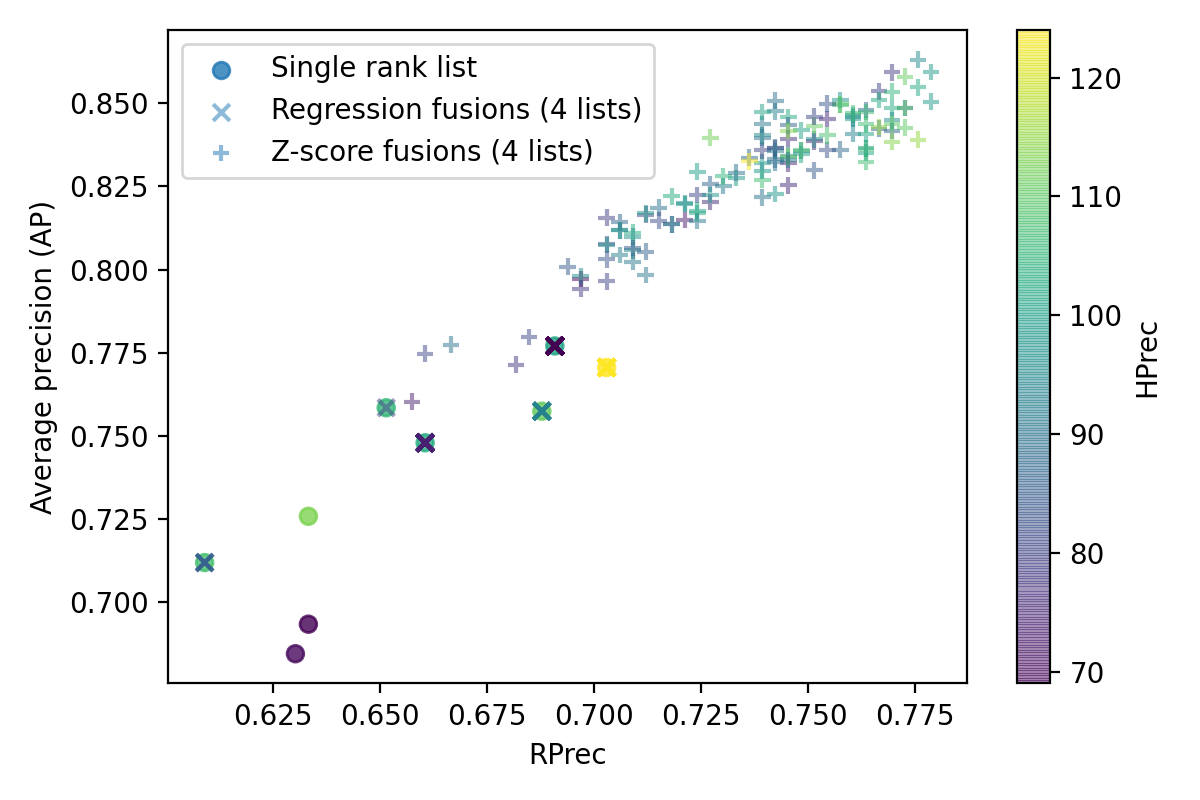
\includegraphics[width=\linewidth]{img/fusion_B_A.png}

  \subcaption{Testing on St-Jean B (training St-Jean A, for the Regression fusion)}
  \label{fig:fusion_A_B}
  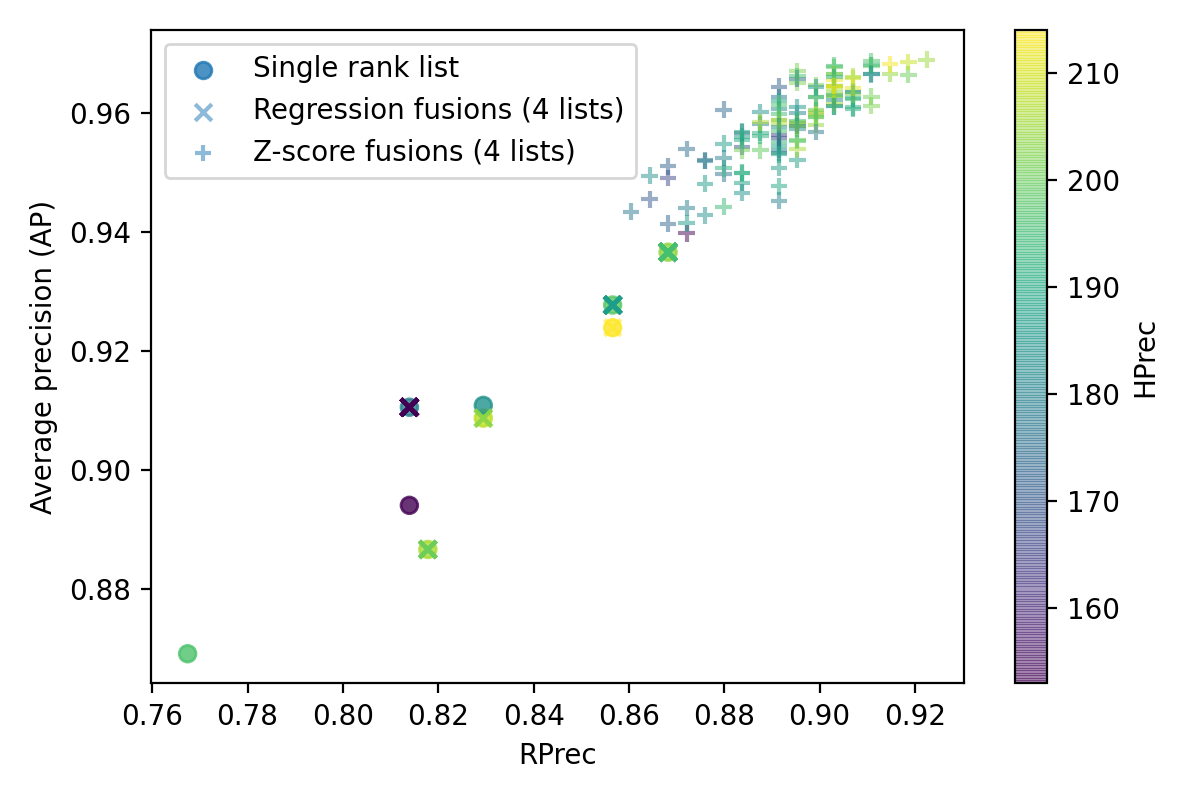
\includegraphics[width=\linewidth]{img/fusion_A_B.png}
\end{figure}

\begin{table}
  \centering
  \caption{Fusion statistics on St-Jean A}
  \label{tab:fusion_stats_A_B}

  \subcaption{Single-Mean}
  \begin{tabular}{l l l l}
    \toprule
    Stats
    & AP
    & RPrec
    & HPrec \\
    \midrule
    Min & $0.704$ & $0.627$ & $42.75$ \\
    Avg$\pm$Std & $0.736\pm0.013$ & $0.656\pm0.012$ & $64.444\pm10.286$ \\
    Max & $0.766$ & $0.686$ & $84.25$ \\
    Argmin & [4,6,7,8] & [4,6,7,8] & [0,1,6,7] \\
    Argmax & [0,2,3,5] & [0,1,2,3] & [2,3,4,8] \\
    \bottomrule
  \end{tabular}

  \subcaption{Single-Max}
  \begin{tabular}{l l l l}
    \toprule
    Stats
    & AP
    & RPrec
    & HPrec \\
    \midrule
    Min & $0.726$ & $0.633$ & $68.0$ \\
    Avg$\pm$Std & $0.769\pm0.009$ & $0.692\pm0.015$ & $88.532\pm9.763$ \\
    Max & $0.777$ & $0.703$ & $99.0$ \\
    Argmin & [4,6,7,8] & [4,6,7,8] & [0,1,6,7] \\
    Argmax & [0,1,2,3] & [0,1,2,3] & [0,1,2,3] \\
    \bottomrule
  \end{tabular}

  \subcaption{Z-Score}
  \begin{tabular}{l l l l}
    \toprule
    Stats
    & AP
    & RPrec
    & HPrec \\
    \midrule
    Min & $0.76$ & $0.658$ & $69.0$ \\
    Avg$\pm$Std & $0.829\pm0.02$ & $0.738\pm0.026$ & $93.833\pm11.108$ \\
    Max & $0.863$ & $0.779$ & $124.0$ \\
    Argmin & [4,5,6,7] & [4,5,6,7] & [0,1,4,5] \\
    Argmax & [0,3,7,8] & [0,3,6,8] & [1,3,6,7] \\
    \bottomrule
  \end{tabular}

  \subcaption{Regression (training St-Jean B)}
  \begin{tabular}{l l l l}
    \toprule
    Stats
    & AP
    & RPrec
    & HPrec \\
    \midrule
    Min & $0.712$ & $0.609$ & $65.0$ \\
    Avg$\pm$Std & $0.764\pm0.016$ & $0.681\pm0.02$ & $72.794\pm12.111$ \\
    Max & $0.777$ & $0.703$ & $99.0$ \\
    Argmin & [4,5,6,7] & [4,5,6,7] & [0,1,2,3] \\
    Argmax & [0,1,2,3] & [2,3,4,5] & [2,3,4,5] \\
    \bottomrule
  \end{tabular}
\end{table}

\begin{table}
  \centering
  \caption{Fusion statistics on St-Jean B}
  \label{tab:fusion_stats_B_A}

  \subcaption{Single-Mean}
  \begin{tabular}{l l l l}
    \toprule
    Stats
    & AP
    & RPrec
    & HPrec \\
    \midrule
    Min          & $0.89$         & $0.80$         & $122.25$      \\
    Avg$\pm$Std & $0.90\pm0.008$ & $0.83\pm0.011$ & $148.11\pm11$ \\
    Max          & $0.92$         & $0.85$         & $172$         \\
    Argmin       & [3,4,7,8]   & [1,3,7,8]   & [1,6,7,8]  \\
    Argmax       & [0,2,5,6]   & [0,2,5,6]   & [0,3,4,5]  \\
    \bottomrule
  \end{tabular}

  \subcaption{Single-Max}
  \begin{tabular}{l l l l}
    \toprule
    Stats
    & AP
    & RPrec
    & HPrec \\
    \midrule
    Min          & $0.91$         & $0.82$         & $153.25$      \\
    Avg$\pm$Std & $0.93\pm0.008$ & $0.86\pm0.012$ & $174.8\pm7$ \\
    Max          & $0.93$         & $0.87$         & $182$         \\
    Argmin       & [3,4,7,8]   & [1,3,7,8]   & [1,6,7,8]  \\
    Argmax       & [0,1,2,3]   & [0,1,2,3]   & [0,1,2,5]  \\
    \bottomrule
  \end{tabular}

  \subcaption{Z-Score}
  \begin{tabular}{l l l l}
    \toprule
    Stats
    & AP
    & RPrec
    & HPrec \\
    \midrule
    Min          & $0.94$         & $0.86$         & $153$      \\
    Avg$\pm$Std & $0.96\pm0.006$ & $0.89\pm0.012$ & $191.3\pm12$ \\
    Max          & $0.97$         & $0.82$         & $214$         \\
    Argmin       & [1,2,3,8]   & [2,3,4,8]   & [1,2,3,8]  \\
    Argmax       & [1,2,5,6]   & [1,2,5,6]   & [2,3,5,7]  \\
    \bottomrule
  \end{tabular}

  \subcaption{Regression (training St-Jean A)}
  \begin{tabular}{l l l l}
    \toprule
    Stats
    & AP
    & RPrec
    & HPrec \\
    \midrule
    Min          & $0.88$         & $0.81$         & $124$      \\
    Avg$\pm$Std & $0.92\pm0.015$ & $0.85\pm0.024$ & $152.9\pm18$ \\
    Max          & $0.94$         & $0.87$         & $182$         \\
    Argmin       & [3,4,5,6]   & [1,2,3,4]   & [1,2,3,4]  \\
    Argmax       & [0,1,2,3]   & [0,1,2,3]   & [5,6,7,8]  \\
    \bottomrule
  \end{tabular}
\end{table}

\begin{table*}
  \centering
  \caption{Rank list fusion sign test. \textit{The star (*) indicate a Binomial test p-value smaller than 5\%}}
  \label{tab:fusion_sign_test}

  \subcaption{Testing St-Jean A (training St-Jean B, for the Regression fusion)}
  \label{tab:fusion_A_B}
  \begin{tabular}{l c c c c}
    \toprule
    Metric
    & Z-Score/T/Single-Mean
    & Z-Score/T/Single-Max
    & Regression/T/Single-Mean
    & Regression/T/Single-Max\\
    \midrule
    AP    & *126/0/0 & *126/0/0  & *108/0/18 & 0/81/45* \\
    RPrec & *126/0/0 & *125/1/0  & *92/4/30  & 0/78/48* \\
    HPrec & *126/0/0 & *111/0/14 & *79/1/46  & 0/14/112*\\
    \bottomrule
  \end{tabular}

  \subcaption{Testing St-Jean B (training St-Jean A, for the Regression fusion)}
  \label{tab:fusion_B_A}
  \begin{tabular}{l c c c c}
    \toprule
    Metric
    & Z-Score/T/Single-Mean
    & Z-Score/T/Single-Max
    & Regression/T/Single-Mean
    & Regression/T/Single-Max \\
    \midrule
    AP    & *126/0/0 & *124/0/2 & *120/0/6  & 0/85/41* \\
    RPrec & *126/0/0 & *119/2/5 & *114/0/12 & 0/76/50* \\
    HPrec & *124/0/2 & *73/3/45 & *92/0/34  & 0/25/101*\\
    \bottomrule
  \end{tabular}

\end{table*}

Using these distance metrics on St-jean, the sign test tends to indicate that the fusion increase the overall quality of the rank list.
The three evaluations metrics are high correlated (especially average precision and R-Precision), only the average precision will be explored in depth.
The Z-Score fusion, produce for every metrics better results than both Single-Mean and Single-Max, the average precision is increase in average by $\sim 10$\% compared to the average of the average precision (Single-Mean) of the rank list used, and by ~6\% in average when considering the maximal average precision (Single-Max).
In the other hand, the Regression fusion, have an average increase of $\sim 3$\% in average precision for the Single-Mean and have a decrease of ~1\% when comparing to the Single-Max.
A general observation of the Tables, show that the HPrec tends to be the least easy metric to increase when using the fusion.
The results of fusing multiple rank lists when using regression fusion strategy tends to indicate that the resulting rank list has in average the same quality as the best rank list used for the fusion with some slight decreases.
This can be further confirmed by looking at Table~\ref{tab:fusion_B_A}, which shows in the column Regression/T/Single-Max more ties than the average and in Figure~\ref{fig:fusions} where most Regression score and and Single rank list score overlap.
No particular set of rank list tends to give the best results in every case when fusing with the two strategies, every rank list is present in the argmax, but with the Z-Score fusion, the best results seem to be obtained with rank lists using different text representations.
The Z-score fusion give the best results overall.

\subsection{Clustering}

\subsubsection{Clustering evaluation metrics}

\begin{definition}[Cluster difference]
  This metric aim to evaluate if the clustering found the right number of cluster.
  The cluster difference is the number cluster found $p$ minus the actual number of cluster $k$.
  \begin{equation}
    Cluster_{diff} = p - k
  \end{equation}
  A positive value indicate an overestimation of the real number of cluster, a negative value indicate the underestimation.
  Zero indicate that the right number of cluster was found.
  This value can be normalized by the number of documents N, which correspond to the difference of the r ratios.
  As stated in the PAN16 evaluation campaign paper, estimating correctly the r ratio tends to indicate a good clustering~\cite{pan16}.
  \begin{equation}
    r_{diff} = \frac{p}{N} - \frac{k}{N} = \frac{p - k}{N}
  \end{equation}
\end{definition}

To evaluate clustering, the metrics used are the BCubed~\cite{bcubed} family (called sometimes $B^3$, in this report).
BCubed has shown to satisfy 4 following importants constraints when evaluating clusterings : \textit{Cluster Homogeneity} (different categories should be in the different clusters), \textit{Cluster Completness} (same categories should belong to the same cluster) and the \textit{Rag Bag constraint} (noisy/miscellaneous categories should be in the same cluster and not in 'healthy' clusters) and the \textit{Cluster size vs quantity constraints} (favorise large cluster)~\cite{bcubed}.
These metrics are used in the clustering task at PAN@CLEF~\cite{pan16}.

\begin{definition}[Correctness~\cite{bcubed}]
  The $BCubed$ metric family is based on the the following \textit{Correctness} principle.
  Let L(e) and C(e) be the category and the cluster of an element e.
  The Correctness is following the biconditional condition on the category and cluster equality (biconditional: $A \Longleftrightarrow B \equiv (A \land B) \lor (\neg A \land \neg B)$).
  \begin{gather*}
    Correctness(e, e') = \\
    \begin{cases}
      1, & if (L(e) = L(e')) \Longleftrightarrow (C(e) = C(e'))\\
      0, & otherwise
    \end{cases}
  \end{gather*}
  In other terms, the correctness has a value of one (100\% correct) if the two elements are in the both in the same cluster and has the same category OR both in a different cluster and a different category.
\end{definition}

\begin{definition}[$BCubed$ Precision~\cite{bcubed}]
  The $BCubed$ Precision correspond to the average of correctness for all elements on the average of all element such that \textbf{their clusters are the same}.
  \begin{equation}
    B^3_{precision} = \text{Avg}_{e}[\text{Avg}_{e' C(e)=C(e')}[Correctness(e, e')]]
  \end{equation}
\end{definition}

\begin{definition}[$BCubed$ Recall~\cite{bcubed}]
  The $BCubed$ Recall correspond to the average of correctness for all elements on the average of all element such that \textbf{their categories are the same}.
  \begin{equation}
    B^3_{recall} = \text{Avg}_{e}[\text{Avg}_{e' L(e)=L(e')}[Correctness(e, e')]]
  \end{equation}
\end{definition}

\begin{definition}[$BCubed F_1$ Score~\cite{bcubed}]
  $BCubed F_1$ Score uses the harmonic mean between the $B^3_{precision}$ and $B^3_{recall}$.
  \begin{equation}
    B^3_{F_1} =
    2 \cdot \frac{B^3_{precision} \cdot B^3_{recall}}
    {B^3_{precision} + B^3_{recall}}
  \end{equation}
  The $F_\beta$ measures, not shown here, provide a parametric way to represent with a single value the two counterbalancing measures in this case, the $B^3_{F_1}$ is computed using the $F$ measures with $\beta = 1$ and the $B^3_{precision}$ and $B^3_{recall}$ scores.
\end{definition}

\subsubsection{Clustering unsupervised cut method}

For this experiment, the goal is to test the unsupervised cut method based on the IPS (Iterative positive silhouette) Procedure on the literature dataset.
When applying the procedure, the number of clusters start at 2, each iteration the silhouette score is computed if it reaches a negative value the procedure stop otherwise the number of cluster is increased and the process is repeated.

The rank list used for this experiment is the one generated using Z-score fusion with retained text representation (9 for St-Jean and 7 for Brunet and Oxquarry), see Section~\ref{sec:annex_retained_text_representation} in annex.

When running the IPS procedure on the dataset, on Figures~\ref{fig:unsupervised_clustering} the silhouette score is indicated as each step and compared to the three BCubed metrics.
For the sake of the experiment, the agglomerative clustering is also run up to a number of cluster equal to the number of documents (singleton clusters).
The detailed score on the unsupervised clustering is presented in Table~\ref{tab:unsupervised_clustering_0}.

Since the rank list used for the clustering is not perfect (every true links at the top), there is no number of cluster with a BCubed $F_1$ score of 1.0.
The estimated number of cluster is on every dataset overestimated, average r-ratio difference of $0.21$, which means that the median neareast-cluster distance is greater than the median intra-cluster distance even when dealing with the right number of clusters.
This can be due to the fact that the rank list used for the clustering is not perfect (AP $\neq 1$).

To mitigate this problem, an easy solution would be to the stop the procedure at for example : $0.1$ instead of $0$.
When running the IPS with a stop at $0.1$ on the dataset, the obtained results are presented in Table~\ref{tab:unsupervised_clustering_01}.
The average r-ratio difference drop to $0.13$ when stopping the procedure at $0.1$ instead of $0$, which seem to improve the results, especially for the Brunet and St-Jean A dataset.
No solid founding are used for tweaking this parameter.

\begin{table}
  \centering
  \caption{Unsupervised clustering evaluation on the datasets}
  \label{tab:unsupervised_clustering}

  \subcaption{IPS Standard Procedure (stop at 0.0)}
  \label{tab:unsupervised_clustering_0}
  \begin{tabular}{l c c c c}
    \toprule
    &
    $B^3_{F_1}$ &
    $B^3_{precision}$  &
    $B^3_{recall}$  &
    $r_{diff}$ \\
    \midrule
    Oxquarry         & 0.73 & 1.00 & 0.58 & 0.23\\
    Brunet           & 0.82 & 0.94 & 0.73 & 0.11\\
    St-Jean A        & 0.64 & 1.00 & 0.47 & 0.22\\
    St-Jean B        & 0.74 & 1.00 & 0.59 & 0.26\\
    \textbf{Average} &
    \textbf{0.73} &
    \textbf{0.99} &
    \textbf{0.59} &
    \textbf{0.21} \\
    \bottomrule
  \end{tabular}

  \subcaption{IPS Procedure with stop at 0.1}
  \label{tab:unsupervised_clustering_01}
  \begin{tabular}{l c c c c}
    \toprule
    &
    $B^3_{F_1}$ &
    $B^3_{precision}$  &
    $B^3_{recall}$  &
    $r_{diff}$ \\
    \midrule
    Oxquarry         & 0.74 & 1.00 & 0.59 & 0.21\\
    Brunet           & 0.82 & 0.82 & 0.82 & 0.05\\
    St-Jean A        & 0.84 & 0.89 & 0.79 & 0.03\\
    St-Jean B        & 0.77 & 1.00 & 0.62 & 0.21\\
    \textbf{Average} &
    \textbf{0.79} &
    \textbf{0.93} &
    \textbf{0.71} &
    \textbf{0.13} \\
    \bottomrule
  \end{tabular}
\end{table}

\begin{figure}
  \caption{Unsupervised clustering example on Brunet and St-Jean B}
  \label{fig:unsupervised_clustering}

  \subcaption{Brunet}
  \label{fig:unsupervised_clustering_brunet}
  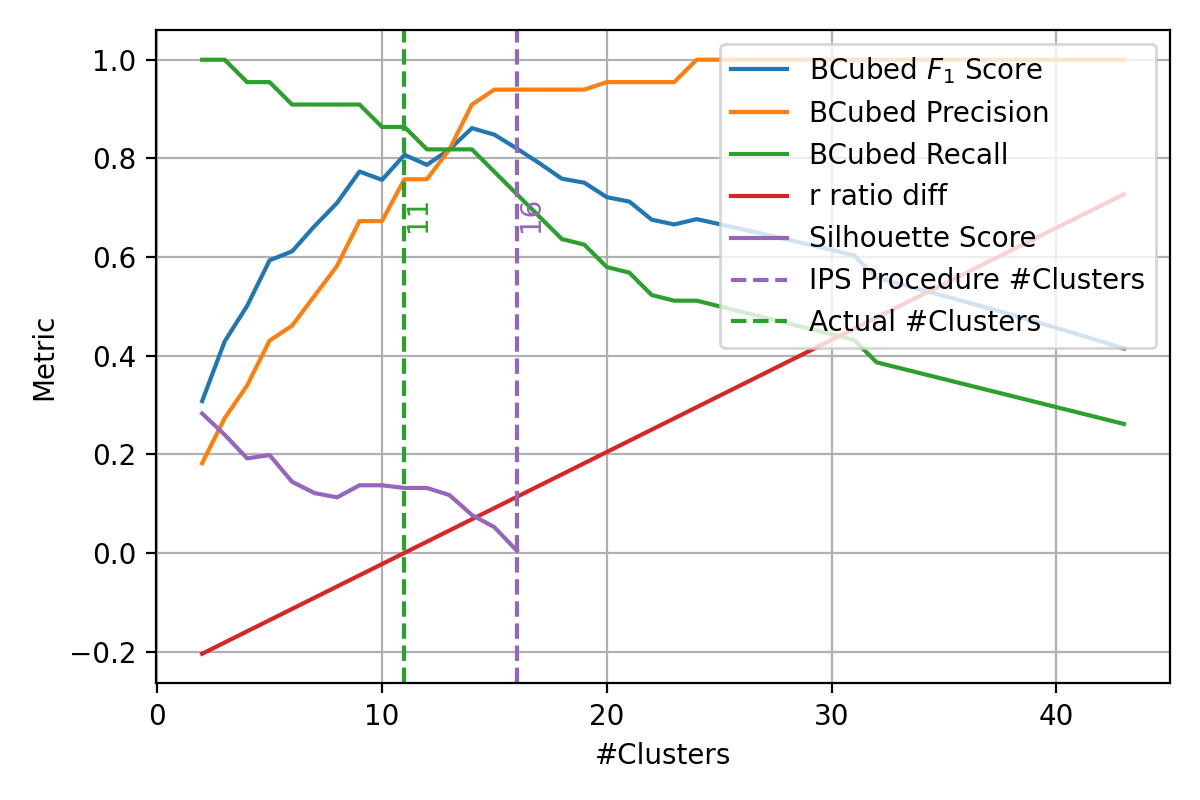
\includegraphics[width=\linewidth]{img/unsupervised_clustering_brunet.png}

  \subcaption{St-Jean B}
  \label{fig:unsupervised_clustering_st_jean_B}
  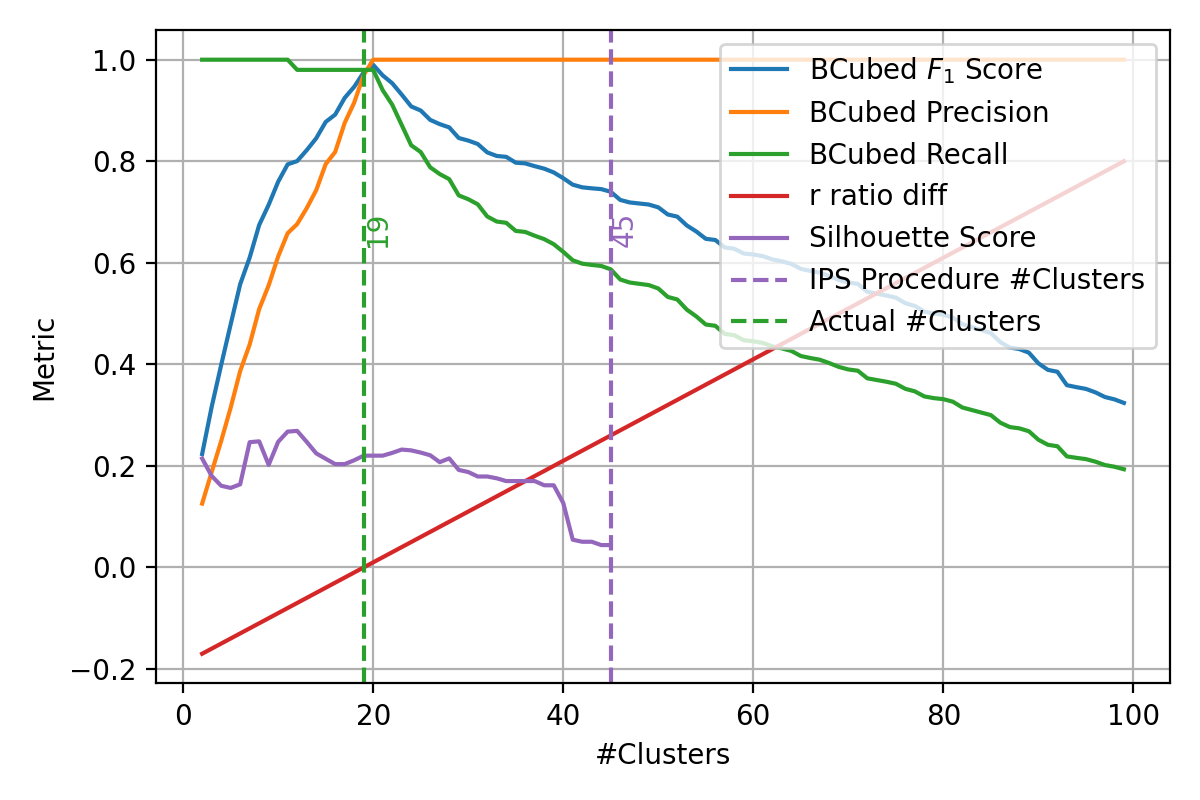
\includegraphics[width=\linewidth]{img/unsupervised_clustering_st_jean_B.png}
\end{figure}

\subsubsection{Clustering with the supervised cut method}

To evaluate the supervised clustering approach, every dataset were used.
First a rank list for each dataset is computed using a z-score fusion using the retained rank list, see Section~\ref{sec:annex_retained_text_representation} in annex.
Then every pair of rank list is used to create a training/testing evaluation.
In other words, a model to create cuts is trained on every dataset and tested on all the datasets.

The model does not depend on the rank list size since only relative magnitudes are used.
The BCubed $F_1$ metrics and the r ratio difference are computed during this experiment and are in presented in Table~\ref{tab:supervised_clustering_train_test}, for every pairs of dataset.
The average values obtained for each metrics is presented in Table~\ref{tab:supervised_clustering_average}.

Multiple points can be observed with these results:
\begin{itemize}
  \item
  When testing the cut model, having a rank list of good quality tends to produce better clustering, no matter the quality of the rank list used for the training.
  \item
  Using the best rank list for training the cut model does not always give the best results.
  An example to illustrate this observation, the St-Jean B dataset have the best rank list with an average precision of 0.97, when using the model trained on this rank list, F1 scores yield by the clustering using this model are : 0.80/0.76/0.82/0.97 (avg: 0.84).
  In the other hand, when using Oxquarry for the training with a rank list of 0.84 AP, the F1 score obtained are : 0.82/0.86/0.88/0.92 (avg: 0.87).
  The Oxquarry dataset seem to be the best dataset to train the model to perform the cut and Brunet the least effective.
\end{itemize}

\begin{table*}
  \centering
  \caption{Supervised clustering evaluation}
  \label{tab:supervised_clustering}

  \subcaption{Every possible training testing dataset pairs. Metrics in order : $B^{3}_{F_1}$ / $B^{3}_{precision}$ / $B^{3}_{recall}$ / $r_{diff}$}
  \label{tab:supervised_clustering_train_test}
  \begin{tabular}{l l| c c c c}
    \toprule
    \multicolumn{2}{c}{\multirow{2}{*}{}} & \multicolumn{4}{c}{Testing} \\
    \multicolumn{2}{c}{} & Oxquarry & Brunet & St-Jean A & St-Jean B \\
    \midrule
    \parbox[t]{2mm}{\multirow{4}{*}{\rotatebox[origin=c]{90}{Training}}}
    & Oxquarry
    & 0.82/1.00/0.70/0.08
    & 0.86/0.91/0.82/0.07
    & 0.88/0.84/0.93/-0.03
    & 0.92/0.88/0.98/-0.02 \\
    & Brunet
    & 0.80/1.00/0.67/0.10
    & 0.75/0.94/0.62/0.18
    & 0.81/0.98/0.69/0.09
    & 0.91/1.00/0.83/0.05 \\
    & St-Jean A
    & 0.80/1.00/0.67/0.10
    & 0.79/0.94/0.68/0.14
    & 0.83/0.89/0.77/0.04
    & 0.97/1.00/0.94/0.02 \\
    & St-Jean B
    & 0.80/1.00/0.67/0.10
    & 0.76/0.94/0.64/0.16
    & 0.82/0.96/0.72/0.07
    & 0.97/1.00/0.94/0.02 \\
    \bottomrule
  \end{tabular}

  \subcaption{Metrics averages}
  \label{tab:supervised_clustering_average}
  \begin{tabular}{l c c c c}
    \toprule
    & $B^{3}_{F_1}$
    & $B^{3}_{precision}$
    & $B^{3}_{recall}$
    & $r_{diff}$ \\
    \midrule
    \textbf{Average}
    & \textbf{0.84}
    & \textbf{0.95}
    & \textbf{0.77}
    & \textbf{0.07}
    \\
    \bottomrule
  \end{tabular}
\end{table*}
